%% (Master) Thesis template
% Template version used: v1.4
%
% Largely adapted from Adrian Nievergelt's template for the ADPS
% (lecture notes) project.


%% We use the memoir class because it offers a many easy to use features.
\documentclass[11pt,a4paper,titlepage]{memoir}

%% Packages
%% ========

%% LaTeX Font encoding -- DO NOT CHANGE
\usepackage[OT1]{fontenc}
%% Babel provides support for languages.  'english' uses British
%% English hyphenation and text snippets like "Figure" and
%% "Theorem". Use the option 'ngerman' if your document is in German.
%% Use 'american' for American English.  Note that if you change this,
%% the next LaTeX run may show spurious errors.  Simply run it again.
%% If they persist, remove the .aux file and try again.
\usepackage[english]{babel}

%% Input encoding 'utf8'. In some cases you might need 'utf8x' for
%% extra symbols. Not all editors, especially on Windows, are UTF-8
%% capable, so you may want to use 'latin1' instead.
\usepackage[utf8]{inputenc}

%% This changes default fonts for both text and math mode to use Herman Zapfs
%% excellent Palatino font.  Do not change this.
\usepackage[sc]{mathpazo}

%% The AMS-LaTeX extensions for mathematical typesetting.  Do not
%% remove.
\usepackage{amsmath,amssymb,amsfonts,mathrsfs}

%% NTheorem is a reimplementation of the AMS Theorem package. This
%% will allow us to typeset theorems like examples, proofs and
%% similar.  Do not remove.
%% NOTE: Must be loaded AFTER amsmath, or the \qed placement will
%% break
\usepackage[amsmath,thmmarks]{ntheorem}

%% LaTeX' own graphics handling
\usepackage{graphicx}

%% We unfortunately need this for the Rules chapter.  Remove it
%% afterwards; or at least NEVER use its underlining features.
\usepackage{soul}

%% This allows you to add .pdf files. It is used to add the
%% declaration of originality.
\usepackage{pdfpages}

%% Some more packages that you may want to use.  Have a look at the
%% file, and consult the package docs for each.
%% See the TeXed file for more explanations

%% [OPT] Multi-rowed cells in tabulars
%\usepackage{multirow}

%% [REC] Intelligent cross reference package. This allows for nice
%% combined references that include the reference and a hint to where
%% to look for it.
\usepackage{varioref}

%% [OPT] Easily changeable quotes with \enquote{Text}
%\usepackage[german=swiss]{csquotes}

%% [REC] Format dates and time depending on locale
\usepackage{datetime}

%% [OPT] Provides a \cancel{} command to stroke through mathematics.
%\usepackage{cancel}

%% [NEED] This allows for additional typesetting tools in mathmode.
%% See its excellent documentation.
\usepackage{mathtools}

%% [ADV] Conditional commands
%\usepackage{ifthen}

%% [OPT] Manual large braces or other delimiters.
%\usepackage{bigdelim, bigstrut}

%% [REC] Alternate vector arrows. Use the command \vv{} to get scaled
%% vector arrows.
\usepackage[h]{esvect}

%% [NEED] Some extensions to tabulars and array environments.
\usepackage{array}

%% [OPT] Postscript support via pstricks graphics package. Very
%% diverse applications.
%\usepackage{pstricks,pst-all}

%% [?] This seems to allow us to define some additional counters.
%\usepackage{etex}

%% [ADV] XY-Pic to typeset some matrix-style graphics
%\usepackage[all]{xy}

%% [OPT] This is needed to generate an index at the end of the
%% document.
%\usepackage{makeidx}

%% [OPT] Fancy package for source code listings.  The template text
%% needs it for some LaTeX snippets; remove/adapt the \lstset when you
%% remove the template content.
\usepackage{listings}
\lstset{language=TeX,basicstyle={\normalfont\ttfamily}}

%% [REC] Fancy character protrusion.  Must be loaded after all fonts.
%% Must be outdated, see https://texwelt.de/fragen/27171/latex-error-command-ifpdftex-already-defined
% \usepackage[activate]{pdfcprot}

%% [REC] Nicer tables.  Read the excellent documentation.
\usepackage{booktabs}

\usepackage{natbib}

\usepackage{textgreek}

\usepackage{caption}

\usepackage{subcaption}

\usepackage{mleftright}     % proper spacing in maths mode

\usepackage{xspace}         % the eater of spaces

\usepackage{siunitx}


%% Our layout configuration.  DO NOT CHANGE.
%% Memoir layout setup

%% NOTE: You are strongly advised not to change any of them unless you
%% know what you are doing.  These settings strongly interact in the
%% final look of the document.

% Dependencies
\usepackage{ETHlogo}

\nonzeroparskip
\parindent=0pt
\defaultlists

% Chapter style redefinition
\makeatletter

\if@twoside
  \pagestyle{Ruled}
  \copypagestyle{chapter}{Ruled}
\else
  \pagestyle{ruled}
  \copypagestyle{chapter}{ruled}
\fi
\makeoddhead{chapter}{}{}{}
\makeevenhead{chapter}{}{}{}
\makeheadrule{chapter}{\textwidth}{0pt}
\copypagestyle{abstract}{empty}

\makechapterstyle{bianchimod}{%
  \chapterstyle{default}
  \renewcommand*{\chapnamefont}{\normalfont\Large}
  \renewcommand*{\chapnumfont}{\normalfont\Large}
  \renewcommand*{\printchaptername}{%
    \chapnamefont\centering\@chapapp}
  \renewcommand*{\printchapternum}{\chapnumfont {\thechapter}}
  \renewcommand*{\chaptitlefont}{\normalfont\huge}
  \renewcommand*{\printchaptertitle}[1]{%
    \hrule\vskip\onelineskip \centering \chaptitlefont\textbf{\vphantom{gyM}##1}\par}
  \renewcommand*{\afterchaptertitle}{\vskip\onelineskip \hrule\vskip
    \afterchapskip}
  \renewcommand*{\printchapternonum}{%
    \vphantom{\chapnumfont {9}}\afterchapternum}}

% Use the newly defined style
\chapterstyle{bianchimod}

\setsecheadstyle{\Large\bfseries}
\setsubsecheadstyle{\large\bfseries}
\setsubsubsecheadstyle{\bfseries}
\setparaheadstyle{\normalsize\bfseries}
\setsubparaheadstyle{\normalsize\itshape}
\setsubparaindent{0pt}

% Set captions to a more separated style for clearness
\captionnamefont{\bfseries\footnotesize}
\captiontitlefont{\footnotesize}
\setlength{\intextsep}{16pt}
\setlength{\belowcaptionskip}{1pt}

% Set section and TOC numbering depth to subsection
\setsecnumdepth{subsection}
\settocdepth{subsection}

%% Titlepage adjustments
\pretitle{\vspace{0pt plus 0.7fill}\begin{center}\HUGE\bfseries}
\posttitle{\end{center}\par}
\preauthor{\par\begin{center}\let\and\\\Large}
\postauthor{\end{center}}
\predate{\par\begin{center}\Large}
\postdate{\end{center}}

\def\@advisors{}
\newcommand{\advisors}[1]{\def\@advisors{#1}}
\def\@department{}
\newcommand{\department}[1]{\def\@department{#1}}
\def\@thesistype{}
\newcommand{\thesistype}[1]{\def\@thesistype{#1}}

\renewcommand{\maketitlehooka}{\noindent\ETHlogo[2in]}

\renewcommand{\maketitlehookb}{\vspace{1in}%
  \par\begin{center}\Large\@thesistype\end{center}}

\renewcommand{\maketitlehookd}{%
  \vfill\par
  \begin{flushright}
    \@advisors\par
    \@department, ETH Z\"urich
  \end{flushright}
}
% Set same size of margins
\setlrmargins{*}{*}{1}
\checkandfixthelayout

% \setlength{\droptitle}{-48pt}

% Turn extra space before chapter headings off.
\setlength{\beforechapskip}{0pt}

\makeatother

% This defines how theorems should look. Best leave as is.
\theoremstyle{plain}
\setlength\theorempostskipamount{0pt}

%%% Local Variables:
%%% mode: latex
%%% TeX-master: "thesis"
%%% End:


%% Theorem environments.  You will have to adapt this for a German
%% thesis.
%% Theorem-like environments

%% This can be changed according to language. You can comment out the ones you
%% don't need.

\numberwithin{equation}{chapter}

%% German theorems
%\newtheorem{satz}{Satz}[chapter]
%\newtheorem{beispiel}[satz]{Beispiel}
%\newtheorem{bemerkung}[satz]{Bemerkung}
%\newtheorem{korrolar}[satz]{Korrolar}
%\newtheorem{definition}[satz]{Definition}
%\newtheorem{lemma}[satz]{Lemma}
%\newtheorem{proposition}[satz]{Proposition}

%% English variants
\newtheorem{theorem}{Theorem}[chapter]
\newtheorem{example}[theorem]{Example}
\newtheorem{remark}[theorem]{Remark}
\newtheorem{corollary}[theorem]{Corollary}
\newtheorem{definition}[theorem]{Definition}
\newtheorem{lemma}[theorem]{Lemma}
\newtheorem{proposition}[theorem]{Proposition}

%% Proof environment with a small square as a "qed" symbol
\theoremstyle{nonumberplain}
\theorembodyfont{\normalfont}
\theoremsymbol{\ensuremath{\square}}
\newtheorem{proof}{Proof}
%\newtheorem{beweis}{Beweis}


%% Helpful macros.
%% Custom commands
%% ===============

%% Special characters for number sets, e.g. real or complex numbers.
\newcommand{\C}{\mathbb{C}}
\newcommand{\K}{\mathbb{K}}
\newcommand{\N}{\mathbb{N}}
\newcommand{\Q}{\mathbb{Q}}
\newcommand{\R}{\mathbb{R}}
\newcommand{\Z}{\mathbb{Z}}
\newcommand{\X}{\mathbb{X}}

%% Fixed/scaling delimiter examples (see mathtools documentation)
\DeclarePairedDelimiter\abs{\lvert}{\rvert}
\DeclarePairedDelimiter\norm{\lVert}{\rVert}

%% Use the alternative epsilon per default and define the old one as \oldepsilon
\let\oldepsilon\epsilon
\renewcommand{\epsilon}{\ensuremath\varepsilon}

%% Also set the alternate phi as default.
\let\oldphi\phi
\renewcommand{\phi}{\ensuremath{\varphi}}

%% Some macros useful for this thesis
\newcommand{\tk}{\text{k}} % kernel function
\newcommand{\td}{\text{d}} % distance function
\newcommand{\MMD}{\text{MMD}} % distance function
\newcommand{\bx}{\mathbf{x}} % distance function
\newcommand{\by}{\mathbf{y}} % distance function

\interfootnotelinepenalty=10000


%% Make document internal hyperlinks wherever possible. (TOC, references)
%% This MUST be loaded after varioref, which is loaded in 'extrapackages'
%% above.  We just load it last to be safe.
\usepackage[linkcolor=black,colorlinks=true,citecolor=black,filecolor=black]{hyperref}


%% Document information
%% ====================

\title{Designing meaningful measures to evaluate generative graph neural networks
on protein datasets.}
\author{Philip Jean Hartout}
\thesistype{Master Thesis}
\advisors{Advisors: Prof. Dr. Karsten M. Borgwardt, Tim Kucera}
\department{Department of Biosystems Science and Engineering}
\date{July 10, 2022}

\begin{document}

\frontmatter

%% Title page is autogenerated from document information above.  DO
%% NOT CHANGE.
\begin{titlingpage}
  \calccentering{\unitlength}
  \begin{adjustwidth*}{\unitlength-24pt}{-\unitlength-24pt}
    \maketitle
  \end{adjustwidth*}
\end{titlingpage}

%% The abstract of your thesis.  Edit the file as needed.
\begin{abstract}
Generative models applied proteins are poised to revolutionize the \emph{in
silico} design of novel proteins satisfying various functional and shape-related
constraints. However, such models are hard to evaluate -- determining how
realistic a generated set of proteins is represents one of the major challenges
in the field of generative models applied to proteins. For graphs, a
representation often used to investigate proteins, the community has gravitated
toward using a kernel two-sample test statistic called the maximum mean
discrepancy. While recent works highlighted some of its pitfalls, this statistic
remains highly versatile since any kernel can be used.

In this thesis, we start by evaluating the expressivity, robustness and
efficiency of maximum mean discrepancy on graph descriptors using graphs
directly extracted from proteins. We then expand the use of MMD by using novel
representations, descriptor functions, and kernels. Specifically, we investigate
the use of graph kernels in MMD. We also devise and apply novel protein-specific
descriptors, such as the dihedral angles histogram formed by each amino acid,
and the pairwise distance histogram of each amino acid, which are both highly
expressive and effecient. Finally, we apply a class of kernels able to operate
on persistence diagrams, a powerful topological descriptor leveraging the
shape-related information in the point clouds formed by each protein structure.


\end{abstract}


%% TOC with the proper setup, do not change.
\cleartorecto
\tableofcontents
\mainmatter

%% Your real content!
\chapter{Introduction}

% Target length: 1,5 pages.

Generative modelling is a highly active branch of machine learning aiming to
model the joint distribution of a certain feature set $x$ and target labels $y$,
often referred to as $p(x,y)$. Modelling this joint distribution presents a lot
of advantages in a myriad of domains, but can be especially
consequential in biology \citep{lopez2020enhancing,strokach2022deep}.

In protein science specifically, the application domains of generative models
can solve a myriad of relevant tasks, from novel protein sequence design, to
designing proteins with specific shapes or functions
\citep{jendrusch2021alphadesign,madani2021deep}. Moreover, the resulting models generate
embeddings and/or weights which can be transferred to discriminative settings
where one seeks to predict $y$ given $x$, i.e. $p(y|x)$. In such a setting, even
more tasks can be tackled using generative models as a starting point, such as protein
structure prediction \citep{jumper2021highly}, function prediction
\citep{meier2021language}, stability prediction \citep{strokach2020fast}.

However, the design and improvement of generative model designs applied to
proteins is prohibited by the lack of suitable evaluation metrics. It is
notoriously hard to find expressive, robust and efficient performance measures
that accurately gauge the quality of generated samples. Efforts have been
made to solve this challenge in the image domain \citep{heusel2017gans}, and
recently, the community has investigated this challenge specifically for a
common representation of proteins: graphs \citep{thompson2022evaluation,
 obray2022evaluation}. In this domain, the standard measure used is a highly
versatile statistic for a kernel two-sample test called \acrfull{mmd}
\citep{gretton2012kernel}.

The results of these investigations, especially those conducted by
\cite{obray2022evaluation}, unveiled a number of pitfalls related to \acrshort{mmd}. Depending
on the kernel and kernel parameter configuration, different \acrshort{mmd} configurations
ranked the quality of samples generated by different models differently. In
addition, when progressively perturbing a set of synthetic graphs, certain \acrshort{mmd}
configurations with respect to another set of unperturbed graphs issued from the
same distribution was not always found to monotonically increase with increasing
amounts of perturbations, casting doubt on the expressivity of \acrshort{mmd} in certain
configurations and data.

In this thesis, we set out to clarify the behaviour of various \acrshort{mmd}
configurations on protein data sets and perform a meta-evaluation of \acrshort{mmd}-based
metrics. We investigate the behaviour of various \acrshort{mmd} configurations by applying
perturbations to one set of proteins. These perturbations are relevant for
protein design use cases and include sequence perturbations, graph perturbations
and geometric perturbations. In this setting, we investigate the behaviour of
classical \acrshort{mmd} configurations typically used to evaluate generative models in the
graph domain. In addition, we expand this set of configurations by devising
novel combinations of protein representations, descriptors, and kernels, all
relevant for different aspects of protein design, and integrate them to the
well-established \acrshort{mmd} evaluation framework.

This thesis is organized as follows: first, Chapter \ref{chap:background}
introduces fundamental concepts that we are going to build upon, and discusses
the surrounding literature. Chapter \ref{chap:methods} details the methodology
of the various experiments that we carry out in this thesis, as well as
describes all the configurations of \acrshort{mmd} that we will explore (i.e. all
combinations of representations, descriptor functions, kernels, and kernel
parameters). Chapter \ref{chap:results} presents and contextualizes the findings of those
experiments. We summarize key findings, make recommendations for practitioners and
highlight some limitations and directions for future work in Chapter
\ref{chap:discussion} before concluding in Chapter \ref{chap:conclusion}.

% Graph representations encapsulates a wide variety of data. Show how they can
% be useful in biology.

% Leslie paper: even worse, depending on parametrization, different models come
% out on top. Call for principled metric design is open.

% Machine learning for graphs. Describe different tasks. Discriminative vs.
% generative modelling.

% Challenges with generative modelling assessment, especially with related to
% graphs vs images. Situate within proteins. Show that it builds on Obray et al.

% Thesis overview

\chapter{Background \& Related Work}

This chapter introduces the core concepts built upon in this thesis and surveys
recent literature tackling the evaluation of generative graph neural networks
and the relevance of this problem in structural biology. Section
[\textbf{REVISE}] defines core mathematical and biological concepts that will
be built upon in the thesis. Section [\textbf{REVISE}] will discuss recent
advances in the design of measures used to evaluate generative graph neural
networks and in structural biology.

The set of methods investigated in this thesis lies at the interface of
structural biology and machine learning. We start by defining some relevant
biological properties of proteins, followed by a survey various graph theoretical
abstractions derived from the protein structure. We then move on to define
generative models and the various classes of measures used to evaluate them.

\section{Proteins}\label{background:proteins}

Proteins are large biomolecules that are formed from a sequence of amino acids,
performing their functions as determined by their three-dimensional structure, and amino
acid sequence. Proteins support a vast array of functions in living organisms,
such as catalysing metabolic reactions, DNA replication, providing structural
support to cells, transporting molecules and sensing stimuli.

Each protein is made up of one or more chains of amino acids, each of which
contain a backbone and different side chains. The atoms in the backbone include
a \textalpha{}-carbon, another carbon and a nitrogen atom. An overview of the
peptide backbone is shown in Figure \ref{fig:backbone}. Interestingly, a plane
is forned by two alpha carbons, the carboxyl group, and the hydrogen atom attached
to the nitrogen atom (see Figure \ref{fig:backbone}), making the peptide bond
between the nitrogen and carbon atom resistant to twisting. That means that the
rotations enabling the 3D folding of a protein is governed by the angle of the bonds linking
the nitrogen atom to the \textalpha{}-carbon and the other carbon atom to the
\textalpha{}-carbon, named \textphi{} and \textpsi{}. These angles' values are
frequently used to validate proteins, characterise the secondary structure of proteins
(i.e. structural features observed in certain segments of proteins), etc.


\begin{figure}[h]
  \centering
  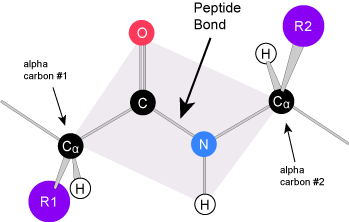
\includegraphics[width=.8\textwidth]{./figures/peptide_bond.png}
  \caption{Schematic of the backbone of a protein. Two \textalpha{}-carbons are
    shown as well as a \textbeta{}-carbon in the middle. R1 and R2 represent the
    side chains of the amino acid. }
  \label{fig:backbone}
\end{figure}


To visualize such angles, a Ramachandran plot can be constructed for any
protein. Such a plot can reveal secondary structural features such as
\textbeta{}-sheets, \textalpha{}-helices, etc. An example of such a plot together
with a 3D model of a protein can be found in Figure \ref{fig:ramachandran}.

\begin{figure}[h]
  \centering
  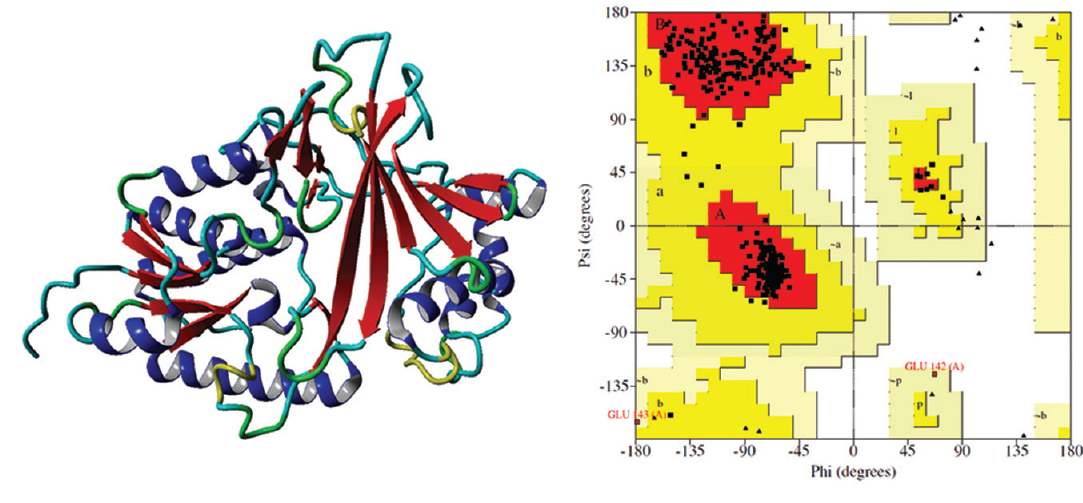
\includegraphics[width=.7\textwidth]{./figures/ramachandran_plot.jpg}
  \caption{3D structure of uridine diphosphogalactofuranose-galactopyranose
mutase with a corresponding Ramachandran plot. The \textalpha{}-helices can be
found on the middle left part of the Ramachandran plot, the \textbeta{} sheets on
the upper right quadrant, and the left handed \textalpha{}-helices can be found in
the middle upper right part of the plot. This figure is adapted from
\cite{nayak2018identification}.}
  \label{fig:ramachandran}
\end{figure}

\section{Graphs}\label{background:graphs}

Proteins are often abstracted using graphs. A graph $G$ is a pair of vertices
$V$ and edges $E$ such that $G=(V, E)$, $|V|=n$ and $|E|=m$. Two vertices $i$
and $j$ are adjacent if there is an edge between them, i.e. $e_{ij}\in E$. The
relationship between between edges can be represented as an $n\times n$
adjacency matrix $A$, where:
\begin{equation}
  \label{eq:adjacency}
  A_{ij}=\begin{cases}
    1, \quad\text{if } e_{ij}\in E\\
    0, \quad\text{otherwise.}
  \end{cases}
\end{equation}
The neighborhood of a node $v$ is the set of nodes with an edge directly to $v$,
i.e. $N(v) = \{ u\in V|e_{uv} \in E \}$. A graph is undirected if the edges do
not contain directional information, i.e. $A_{ij}=A_{ji}$. A directed graph
would result in directionality being encoded in edges, where $A_{ij}$ would not
contain any information about $A_{ji}$. Nodes and edges in each graph can
contain one or more labels. In this thesis, we will mostly deal with labeled
undirected graphs, where each node will be labeled according to the amino acid
type each node belongs to.

There are multiple ways of constructing graphs from proteins. First, one can
extract a \emph{contact map} of a protein by computing the (euclidean) distance
between any two points belonging to each amino acid. The \textalpha-carbon is
often used for this purpose. This is a fully connected graph with continuously
labeled edges representing the distance between each node. From there, it is
possible to either extract a $k$-nearest neighbour graph, where
$k\in\mathbb{N}>0$ defines the amount of nodes directly connected to any given
nodes; or an $\varepsilon$-graph, where each node within a given distance
$\varepsilon\in\mathbb{R^+}\setminus \{0\}$ of another node is connected. Both
are graphs where each node is labeled with the residue name to which the
\textalpha{}-carbon belongs and the edges are unlabeled.

\section{Topological Data Analysis}

Although graphs are powerful representation of proteins, the latter can also be
represented as \emph{point clouds}. One powerful field of study of topological
properties of point clouds is \emph{topological data analysis}.

Topology has witnessed relentless theoretical progress since Henri Poincaré
first addressed topological ideas as a distinct branch of mathematics in his
1895 publication of \textit{Analysis Situs}~\citep{poincare1895analysis}. Only
recently, -- with the advent of modern computing -- has the field of
computational topology and topological data analysis (TDA) gained momentum to
investigate (high-dimensional) data in physics, biology, and
beyond~\citep{dey1999computational, ghrist2008barcodes, amezquita2020shape}. For
material providing an extensive and formal introduction to topology and
persistent homology, please refer to~\citep{freedman2009algebraic,
edelsbrunner2010computational}, and \citep{ghrist2008barcodes}.

A powerful computational technique to analyse topological properties of point
clouds is \emph{persistent homology}, which first requires us to define
simplicial homology. Simplicial homology refers to a way of assigning
connectivity information to topological objects, such as point clouds, which are
represented by simplicial complexes. A simplicial complex $K$ is a set of
simplices which correspond to vertices in dimension 0, edges in dimension 1 and
triangles in dimension 2. The subsets of a simplex $\sigma\in K$ are referred to
as its faces, and every face $\tau\in K$. Moreover, any non-empty intersection
of two simplices also needs to be part of the simplicial complex, i.e.
$\sigma\cap\sigma '\neq\emptyset$ for $\sigma,\sigma '\in K$ implies
$\sigma\cap\sigma'\in K$, meaning that $K$ is closed under calculating the faces
of a simplex.

Persistent homology extends simplicial homology by employing filtrations to
imbue $K$ with scale information. This process captures rich, mutli-scale
topological information related to $K$ in a principled way. The filtration
process is generally defined by a function $f: K\to\mathbb{R}$ satisfying some
finite number of values $m$ and $f^{0}\leq f^{1}\leq\dots\leq f^{m-1}\leq
f^{m}$. This allows us to sort $K$ using $f$, for instance by extending $f$
linearly to higher-dimensional simplices via $f(\sigma):=\max_{v\in\sigma}f(v)$,
leading to a nested sequence of simplicial complexes like so:
\begin{equation}
  \label{eq:nested_simplicial_complexes}
  \emptyset=K^{(0)}\subseteq K^{(1)}\subseteq \dots\subseteq K^{(m-1)}\subseteq K^{(m)},
\end{equation}
where $K^{(i)}:=\{\sigma\in K\ |\ f(\sigma)\leq f^{(i)}\}$. This relationship
enables tracking the appearance (i.e. a connected component arising) and the
dissapearance (i.e. two connected components into one) of topological features
across scales as one transitions from $K^{(i)}$ to $K^{(i+1)}$. The birth (i.e.
appearance) and death (i.e. dissapearance) of topological features for different
values of $f$ are usually summarized in a \emph{persistence diagram}, which is a
multiset of tuples, each of which contains the values at which each features is
born or dies.

A common construction for obtaining such features is the Vietoris-Rips complex
\citep{vietoris1927hoheren}. It requires a distance threshold $\varepsilon$ and
a metric $\text{d}( \cdot, \cdot)$ (usually, the Euclidean distance, as we will
use in this thesis). The Vietoris-Rips complex at scale $\varepsilon$ of an
input protein point cloud is defined as
$\mathcal{V}_{\varepsilon}(X):=\{\sigma\subseteq X| \text{d}(x(i),
x(j))\leq\varepsilon\},\ \forall x(i),x(j)\in\sigma$, i.e.
$\mathcal{V}_{\varepsilon}$ contains all subsets of the input space whose
pairwise distances are less than or equal to $\varepsilon$.
$\mathcal{V}_{\varepsilon}$ is conceptually very similar to the
$\varepsilon$-graphs discussed in section \ref{background:graphs}, except that
$\varepsilon$ here ranges over the entire space of possible distance values, and
$\mathcal{V}_{\epsilon}$ also tracks topological features over all three
dimensions, instead of only connected nodes\footnote{Technically, since our
input consists of points (a.k.a. 0-simplicial complexes) exclusively (and not 1-
or 2- simplicial complexes), we are actually primarily concerned with a
subcomplex of $\mathcal{V}_{\varepsilon}(X)$ called the \v{C}ech complex.}.

Note that the multiplicity of the persistence diagram corresponds to the number
of homology dimensions under study. In this thesis, given proteins are
represented as three-dimensional point clouds, we choose to track topological
features across three homology dimension: 0,1 and 2. Effectively, this tracks
connected components in dimension 0, circular holes in dimension 1 and two
dimensional voids or cavities in dimension 2 as the filtration function is
applied. For a more thorough introduction to homology and homology groups,
please refer to \citet{edelsbrunner2010computational}.

\section{Generative models}

This thesis deals with measures to assess generative model performance, so we
define generative models here. While discriminative machine learning techniques
aim to learn some dependent variable $\mathcal{Y}$ from a set of (independent)
features $\mathcal{X}$, generative machine learning models generate synthetic
samples $\mathcal{X}'$ following the distribution of $\mathcal{X}$. Computing
such probabilistic distributions through maximum likelihood estimation and
related methods is intractable in many cases; as such, new learning paradigms
were established to enable the modeling of complex, real-world distributions
through gradient-based methods.

One such seminal method was that of generative adversarial learning, pioneered
by \citet{goodfellow2014generative}, where a (deep) generator is pitted against
a (deep) discriminator. The former's goal is to generate samples identical to
the training distribution, while the latter is to classify whether or not the
sample originated from the generator or the training distribution.
Simultaneously developed methods by \citet{kingma2013auto} generalized this idea
further and introduced the variational auto-encoder, where instead of a
discriminator, the second network leverages the representation of the generator
to perform approximate inference. In both cases, the two networks (i.e. the
generator and the discriminator/inference network) are jointly trained using
backpropagation to minimize some appropriate loss function.

\textbf{[ADD LOSS FUNCTIONS]}

A recent review of the existing landscape of generative modelling methods has
been provided by \citet{bond2021deep}.

These techniques have been particularly successful in the image domain, where
modern GANs have been able to tackle multiple practical challenges such as mode
collapse and convergence failure to produce realistic images, such as the sample
seen in Figure \ref{fig:styleganxl}. More pertinent to this thesis is the
application of generative models to graphs. The application domain has been
reviewed by \citet{zhou2020graph}. In short, graph generative networks are
capable of operating on the highly versatile and extensible graph domain. It has
been shown that they can produce small molecules, generate social networks,
knowledge graphs, among many other real-world tasks. Generative networks can be
grouped into two categories: those that generate nodes in each graph
sequentially, such as GraphRNN by \cite{you2018graphrnn}, and those that generate
graphs from some latent distribution directly, such as MolGAN by
\cite{de2018molgan}.

\begin{figure}
  \centering
  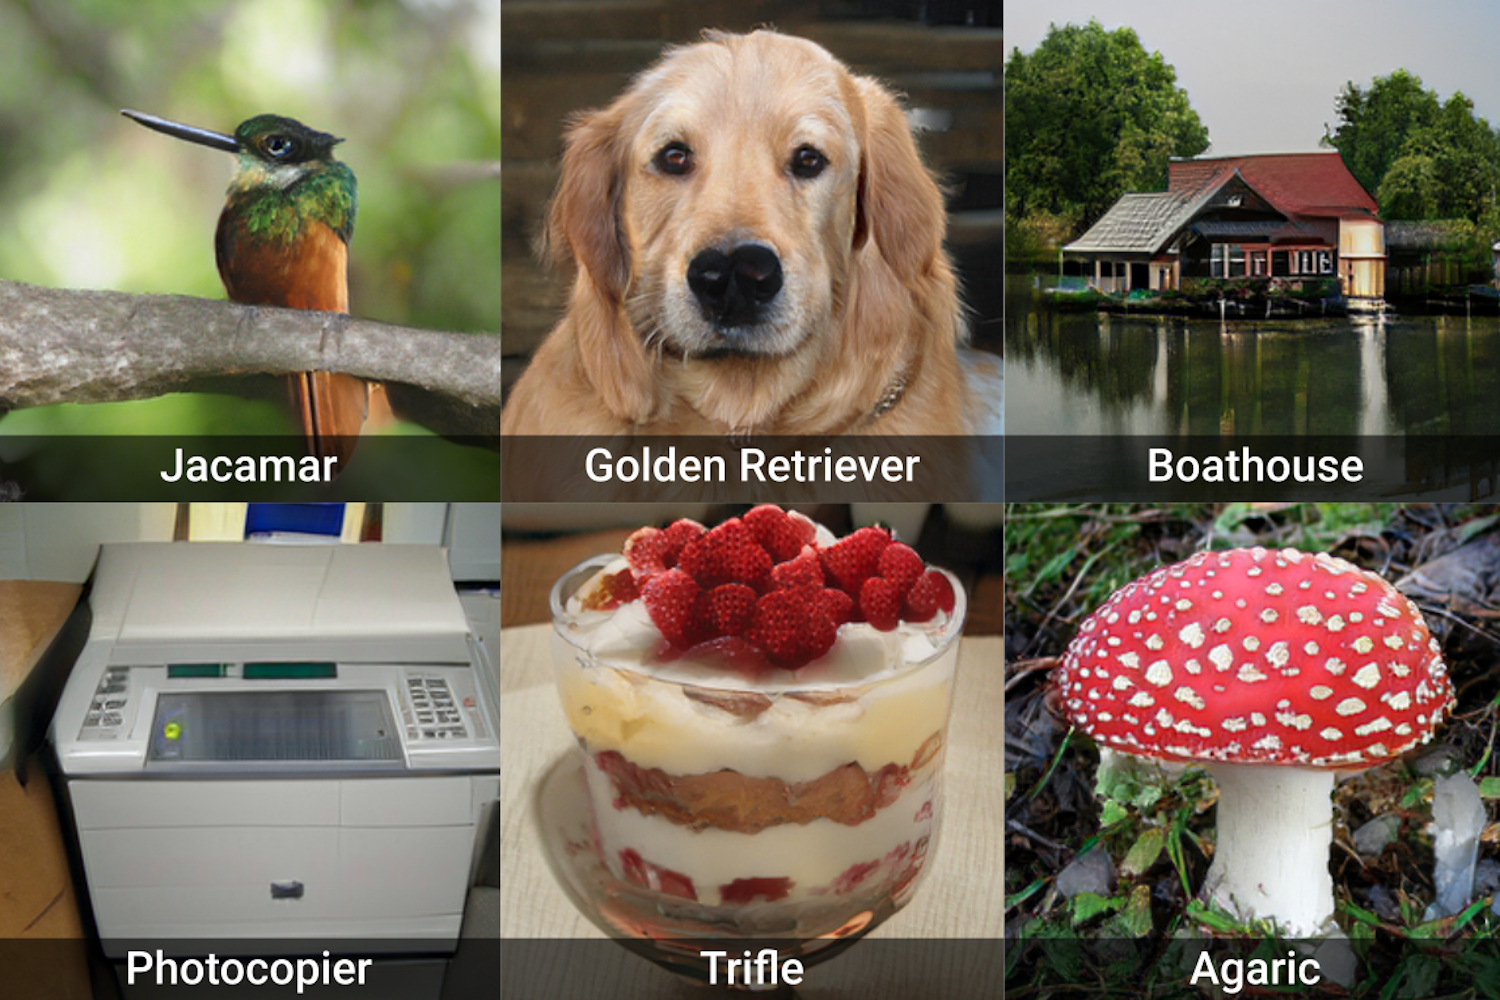
\includegraphics[width=0.7\textwidth]{./figures/representative_image.jpg}
  \caption{Sample images generated by StyleGAN-XL, the state-of-the-art GAN
by \citet{sauer2022stylegan} at the time of writing.}
  \label{fig:styleganxl}
\end{figure}

Operating in the graph domain incurs some unique challenges. From a modelling
standpoint, dealing with graphs means dealing with a much larger and variable
output space. Specifically, when dealing when an undirected graph of $n$ nodes,
at least $n^2/2$ values need to be specified. Additionally, the number of edges
and nodes vary from sample to sample, which also needs to be accounted for in
the model structure. Additionally, building a generative model generating graphs
of up to $n$ nodes, $n!$ possible adjacency matrices can be generated. Such a
high representation complexity is challenging to model, expensive to
compute, and difficult for objective functions to optimize. The last
modelling-related issue when dealing with graphs is that the presence of one
edge is not independent from another, i.e. real-world graphs often exhibit
patterns of local connectedness which need to be accounted for in the model.

But perhaps the most significant problem plaguing all generative models is the
evaluation problem. Concretely, this problem can be framed using the following
question: how does the practitioner go about evaluating the quality of
the set of samples generated? While sidestepping the problem is possible in the image
domain by manually inspecting generated samples, a practice that might reveal
interesting modelling pathologies, this cannot be done at scale, and for
generative models operating in the graph domain.



\section{Maximum Mean Discrepancy \& Kernel methods}\label{background:kernels}

% \section{Related Work}\label{sec:related}

% \subsection{Structural Biology}

% \subsection{Metrics for Generative Graph Models}

\section{Summary}

\chapter{Methods}\label{chap:methods}

The primary methodology employed in this thesis to assess the quality of metrics
used to evaluate generative protein models follows a fundamentally similar
approach used by \cite{o2021evaluation}, which we adapt to include the following
steps:

\begin{enumerate}
\item Take two i.i.d. samples a database of proteins.
\item Progressively add some perturbation to one of the samples.
\item Measure the MMD between the unperturbed and perturbed sample.
\end{enumerate}

We start by motivating the datasets that will be used to simulate a generative
protein model. We then describe and motivate the experimental setups -- i.e.
perturbations -- that we will employ to test the various configurations MMD.
Finally, we enumerate and justify which configurations of MMD are tested,
including all the combinations of protein representations, descriptor functions,
and kernels. Finally, we describe and motivate the experimental setups -- i.e.
perturbations -- that we will employ to test the various metric configurations.


\section{Datasets}

Because generative models have not been applied to proteins yet, which is partly
due to the lack of suitable evaluation metrics, no generative model can be used
here. In this thesis, except otherwise stated, all results will be dervied from
10 random samples from the \textit{homo sapiens} monomeric proteome downloaded
from the EBI AlphaFold2 database
\citep{varadi2022alphafold,tunyasuvunakool2021highly}, a repository comprising
predicted 3D structures of protein sequences obtained from AlphaFold2, the
current state-of-the-art method to predict protein structure from sequences
\citep{jumper2021highly}. This dataset was chosen because it contains
consistently formatted \texttt{pdb} files only containing information from
heavy atom directly contributing to the 3D structure of a single monomer, which
simplifies downstream processing.

\section{Perturbations}

While \cite{o2021evaluation} focused on \emph{graph perturbations} specifically,
we wanted to augment and refine the set of perturbation applied to the perturbed
sample of proteins to be more pertinent to proteins. Three
categories of perturbations can be distinguished:

\paragraph{Graph Perturbations} These perturbations mostly overlap with those
defined by \cite{o2021evaluation}, as they include (i) adding edges to a graph
(ii) removing edges from a graph (iii) rewiring, i.e. swapping, edges within a
graph.
\paragraph{Point cloud perturbations} These perturbations aim to add changes
to the underlying coordinates of each of the atom in the protein. Such
perturbations include injecting Gaussian noise (Equation
\ref{eq:gaussian_noise}), (ii) twisting, , (iii) shearing, and
(iv) tapering. We proceed to detailing each of the equations governing the
perturbations below. An illustration of each of those perturbation can be found
in Figure \ref{fig:perturbation_illustration}

In the notations that follow, $x$, $y$ $z$ represent the unperturbed coordinates, and
$x'$, $y'$, and $z'$ represent the perturbed coordinates. The Gaussian noise added to a coordinate system is given by:
\begin{equation}
  \label{eq:gaussian_noise}
  \begin{bmatrix}
    x' \\
    y' \\
    z'
  \end{bmatrix} =
  \begin{bmatrix}
    x + \sigma \\
    y+ \sigma \\
    z+ \sigma
  \end{bmatrix}
\end{equation}
where $\sigma\sim\caln(0,\sigma)$ is set by the user. Twisting is achieved by
adding the following transformation to the coordinate system:

\begin{equation}
  \label{eq:twisting}
  \begin{bmatrix}
    x' \\
    y' \\
    z'
  \end{bmatrix} =
  \begin{bmatrix}
    x\cdot\cos(\alpha\cdot z) - y\cdot\sin(\alpha\cdot z) \\
    x\cdot\sin(\alpha\cdot z) + y\cdot\sin(\alpha\cdot z) \\
    z
  \end{bmatrix}
\end{equation}

where $\alpha\in\R$ is in $\rad\cdot\si{
\angstrom}^{-1}$ is set by the user. Shearing the coordinate system is achieved
by applying

\begin{equation}
  \label{eq:shearing}
  \begin{bmatrix}
    x' \\
    y' \\
    z'
  \end{bmatrix} =
  \begin{bmatrix}
    a \cdot z + x\\
    b \cdot z + y\\
    z
  \end{bmatrix}
\end{equation}

to the coordinate system, where $a, b\in\R$ are in \si{\angstrom} and set by the user. In this thesis, we set $a=b$. Similarly,
tapering is achieved by applying


\begin{equation}
  \label{eq:tapering}
  \begin{bmatrix}
    x' \\
    y' \\
    z'
  \end{bmatrix} =
  \begin{bmatrix}
    (0.5\cdot a^2\cdot z + b\cdot z + 1) \cdot x\\
    (0.5\cdot a^2\cdot z + b\cdot z + 1) \cdot y\\
    z
  \end{bmatrix}
\end{equation}

where $a, b\in\R$ are in \si{\angstrom} and set by the user. Similarly to
Equation \ref{eq:shearing}, we set $a=b$ in this thesis.

\begin{figure}
  \centering
  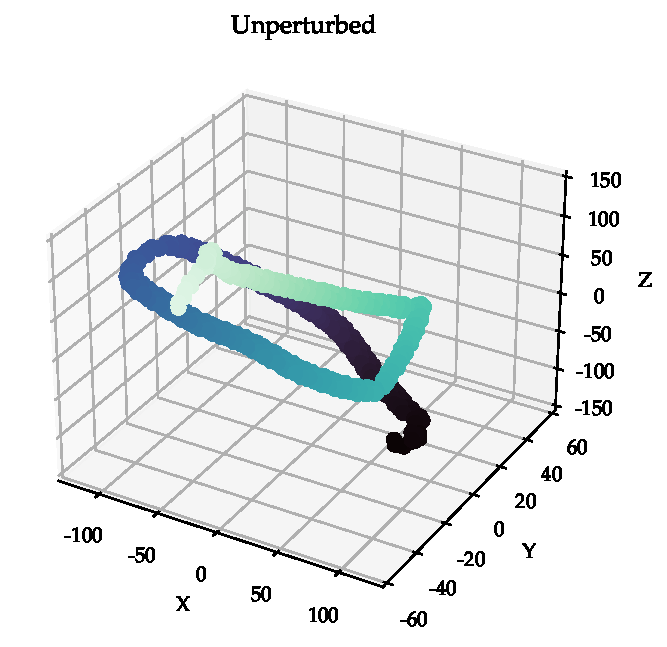
\includegraphics[width=0.5\textwidth]{./figures/protein_unperturbed.pdf}
  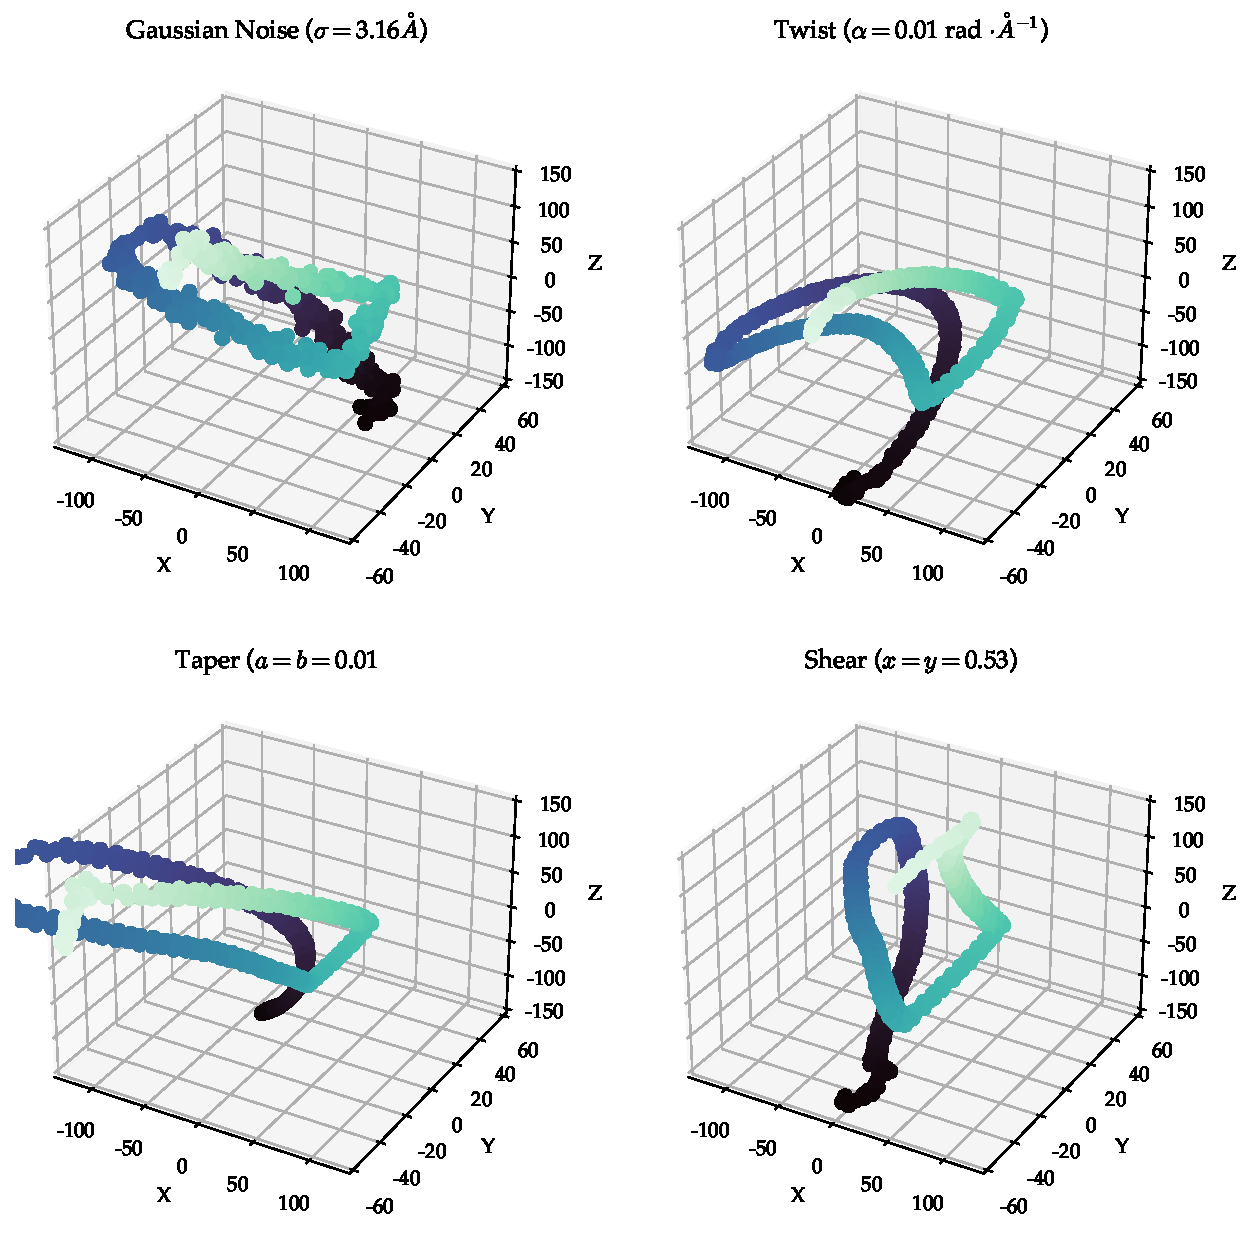
\includegraphics[width=\textwidth]{./figures/protein_perturbed.pdf}
  \caption[Illustration of the perturbations applied to proteins.]{Illustration
of the perturbations applied to proteins. The protein displayed here is the
Cilia- and flagella-associated protein 53 (PDB entry: Q96M91). Each $\alpha$
carbon is colored according to its position on the chain. On the unperturbed
protein, the lighter colors are located closer to the viewer.}
  \label{fig:perturbation_illustration}
\end{figure}

\paragraph{Mutation} These simply consist in swapping node labels, i.e.
changing an existing node label, with another. While graph perturbation
probabilities (e.g. of adding an edge) ranges from 0 to 1, here we mostly
concentrate on lower regimes of mutation, i.e. between 0 and 0.1, so see how
sensitive the MMD to a few point mutations, which covers some of the
real-world protein engineering use cases \citep{poluri2016protein}.

For each perturbation, a range of degree of perturbation is defined and 20
different evenly-spaced degrees of perturbation is examined and repeated 10
times with 10 pairs of i.i.d. proteins to estimate the sensitivity of the
particular MMD configuration to the perturbation. The ranges used for each
parameter used in this thesis is shown in Table \ref{tab:perturbation_ranges}


\begin{table}
  \centering
  \begin{tabular}{>{\raggedright\arraybackslash}p{4.8cm}l}
    \toprule
    \textbf{Perturbation} & \textbf{Range} \\
    \midrule
    Twist & [0, 0.1] (rad/\si{\angstrom})\\
    Shear & [0, 5] (\si{\angstrom}) \\
    Taper & [0, 0.1] (\si{\angstrom}, \si{\angstrom}) \\
    Gaussian Noise & [0, 30] (\si{\angstrom}) \\
    Mutation & [0, 0.1]\\
    Graph Perturbations (remove, add, rewire edges) & [0, 1]\\
    \bottomrule
  \end{tabular}
  \caption{Perturbation ranges used in this thesis. Each interval was split into
    20 evenly-spaced degrees of perturbation.}
  \label{tab:perturbation_ranges}
\end{table}

\section{MMD Configurations}

We introduced MMD in Section \ref{sec:mmd}, Equation \ref{eq:mmd}, and
noted that an important part of MMD consists in choosing the right set of
descriptor function and kernel. Here, we list and motivate all graph extraction techniques,
descriptor functions employed, and kernels adopted in this experiment.

First, throughout our experiments we will use the unbiased squared MMD estimate,
which removes self-comparison terms in the kernel matrices
(\cite{gretton2012kernel}, Lemma 6), which can result in negative values. We
will normalize the resulting MMD over the whole range of perturbation for each
curve as well to compare behaviours of different MMD configurations not
operating on the same scale.

\begin{equation}
  \label{eq:normalization}
  \MMD_{\textnormal{Normalized}} = {\MMD - \min(\MMD_{\textnormal{Experiment}}) \over \max(\MMD_{\textnormal{Experiment}}) - \min(\MMD_{\textnormal{Experiment}})}
\end{equation}

Where $\MMD_{\textnormal{Experiment}}$ is the collection of MMD values for a particular
experiment, i.e. a particular MMD configuration tracked through the whole range
of a particular perturbation.

\subsection{Representations}
We will use several different representations in this thesis, which can be
grouped into three categories. The first is \emph{coordinates}. These are parsed
from each \texttt{.pdb} file. The second is \emph{graphs}. They include $k$-NN
and $\varepsilon$-graphs, introduced in Section \ref{sec:graphs}. A summary
table of the different types of graphs extracted from proteins in this thesis
can be found in Table \ref{tab:graph_extraction}. The third is the simple
protein \emph{sequence}. Each protein's sequence parsed from each \texttt{.pdb}
file as is. Since we are only dealing with monomers, no additional processing is
required.

\begin{table}
  \centering
  \begin{tabular}{ll}
    \toprule
    \textbf{Graph type} & \textbf{Values} \\
    \midrule
    $k$-NN graphs & 2, 6, 8 \\
    $\varepsilon$-graphs & 8, 16, 32 \\
    \bottomrule
  \end{tabular}
  \caption{Ranges of parameters used to extract graphs from point clouds in this thesis.}
  \label{tab:graph_extraction}
\end{table}


\subsection{Descriptor functions}\label{sec:descriptors}

As discussed Section \ref{sec:mmd}, some kernels require some alternative vectorized
representation to work. We will use the following protein descriptor functions
here.


\paragraph{Graph descriptors} They are defined in Section \ref{sec:mmd} and include
  the degree distribution histogram, the clustering coefficient histogram and
  the laplacian spectrum histogram. These are all fixed-length vectors. Of note,
  we let the degree histogram in a range of 2699, due to the fact that adding
  edges between all nodes of the longest protein containing 2699 residues will
  result in the highest-degree node to be 2698.
\paragraph{Coordinates descriptors} In order to capture the information of the
3D structure of the protein beyond local neighbourhood information, a
topological descriptor of each protein in the form of a persistence diagram is
extracted using a Vietoris-Rips filtration introduced in detail in Section
\ref{sec:tda}. To speed up computation, we sampled every other point to
dramatically reduce the running time and memory footprint without significantly
affecting the shape of the protein.
\paragraph{Protein-specific descriptors} In this thesis we introduce two novel
protein-specific descriptor functions resulting in fixed-length vector
representations. The first consists in a histogram of the pairwise distance of
each atom considered; the second consists in concatenating the two histograms of
the two dihedral angles $\phi$ and $\psi$ formed by each amino acid discussed in
Section \ref{sec:proteins}. The inspiration behind those two descriptors comes
from elements of the validation pipeline of novel Protein Data Bank structures
\citep{read2011new, gore2012implementing, gore2017validation}, where atoms too
close together are flagged and unusual dihedral angles are reported. Those
unusual dihedral angles are also called ``Ramachandran outliers'', after the
scientist who discovered a way to display the $\phi$ and $\psi$ in a 2-D
histogram, and recovered items related to the secondary structure of the protein
from such plots. \citep{ramachandran1063Stereochemistry}.

\paragraph{Sequence descriptors} In Section \ref{sec:mmd}, we discussed the
Evolutionary Scale Modelling family to construct descriptors of a fixed length
using a learned embedding. We are going to use the 6-layer variant trained on
the UniRef50 snapshot from March 2018 containing approximately 43 million
parameters, because it is able to process the full range of sequence lengths
that we have in our dataset (the longest sequence fragment is 2699 amino acids long).

Table \ref{tab:descriptor_function_setup} summarizes the parameters used to set
up the descriptor functions in this thesis.

\begin{table}
  \centering
  \begin{tabular}{lll}
    \toprule
    \textbf{Descriptor Name} & \textbf{Number of Bins} & \textbf{Range of Bins} \\
    \midrule
    Degree Histogram & 2699 & [0, 2699] \\
    Laplacian Spectrum Histogram & 100 & [0, 2] \\
    Distance Histogram & 1000 & [0, 1000] (\si{\angstrom}) \\
    Dihedral Angles Histogram & 100 & [$-\pi$, $+\pi$] (rad) \\
    \bottomrule
  \end{tabular}
  \caption[Descriptor function bin numbers and ranges of descriptor functions
  used in this thesis.]{Descriptor function bin numbers and ranges of descriptor functions
    used in this thesis. The ranges are given by
    [minimum value, maximum value] and (unit) when applicable.}
  \label{tab:descriptor_function_setup}
\end{table}

% TODO: add pgfplots figure of this workflow.

\subsection{Kernels}\label{sec:methods_kernels}
Once a suitable representation and descriptor function is selected, one requires
a kernel to evaluate the MMD in the corresponding RKHS. We detail which kernels
we are going to evaluate and why in this section. Kernels used in this thesis can be grouped into
three separate categories.

The first category has been discussed in the literature extensively since it was
used to evaluate generative graph neural network models, i.e. the
\emph{fixed-length vector kernels} like the Gaussian (RBF) kernel and the linear
kernel, both of which are defined in Section \ref{sec:kernels}\footnote{We will
  follow the speed up trick outlined in Appendix A.5 by \cite{o2021evaluation}
  to reduce the computation time of each different bandwidth parameter}. Since the only
condition for each vector to be valid inputs for those kernels is that they are
in $\R^d$, the protein-specific vector representations outlined in Section
\ref{sec:descriptors} are valid inputs.
% Special implementation of wl-k

As aluded to in Section \ref{sec:kernels}, we introduce two new classes of
kernels for use in MMD which so far have not been used to evaluate generative
models due to the unique aspects of proteins that need to be captured. This
brings us to the second category of kernels used in this thesis: \emph{graph kernels}.
Specifically, we are going to use the Weisfeiler-Lehman kernel discussed in
Section \ref{sec:kernels} because it captures \emph{local} patterns in the
neighbourhood of each node. In Appendix \ref{sec:sparse_wl}, we detail how we
achieved an 80\% improvement in runtime of the Weisfeiler-Lehman kernel by
leveraging the sparsity of the graphs used in this thesis.

To estimate \emph{global} changes in the shape of the protein, we will also use
kernels using persistence diagrams as input, specifically using the Persistence
Fisher kernel defined in Section \ref{sec:kernels} \citep{le2018persistence}.


\section{Experimental Setup}

\subsection{Measuring the quality of MMD configurations}

To objectively evaluate the various representation, descriptor, and kernel
combinations used in MMD, we will use two correlation coefficients, namely the
Spearman's correlation coefficient and Pearson's correlation coefficient, each
given by:
\begin{equation}
  \label{eq:spearman} \rho_p(X,Y) = {\cov(\rank(X), \rank(Y)) \over
\sigma_{\rank(X)}\sigma_{\rank(Y)}},
\end{equation} and
\begin{equation}
  \label{eq:pearson} \rho_s(X,Y) = {\cov(X, Y)\over \sigma_X\sigma_Y},
\end{equation}
respectively. Here, $X$ is the vector containing the ordered set of values used
to perturb one of the protein sets and $Y$ the vector of ordered MMD values
between the unperturbed and perturbed set for each perturbation level. In this
setting, a high Spearman correlation coefficient (Equation \ref{eq:spearman}) is
crucial to satisfy the first criterium of a performance metric: expressivity
(see Section \ref{sec:evalproblem}). This will guarantee that the metric
increases monotonically with the amount of perturbation. As
\cite{o2021evaluation} have showed, some configurations of MMD on synthetic
datasets showed that an increasing MMD value with increasing perturbation is not
guaranteed. While \cite{thompson2022evaluation} highlighted that linearity is
not a requirement, the Pearson correlation coefficient (Equation
\ref{eq:pearson}) will allow us to further refine the selection of the metrics
behaving most predictably, and distill the most relevant configurations for a
given perturbation range.

\subsection{Software Library Design}


Due to the complexity and modularity of the methodology outlined above, it is
required to have a scalable library to execute all the evaluation experiments at
scale and efficiently. To accomplish this task, we developed a custom Python
library leveraging parallel processing of data to the greatest extent possible.
We were inspired by the standards of \texttt{scikit-learn} and implemented
multiple modules following the same design patterns to ensure that we could
build \texttt{Pipeline} objects with the necessary steps required to compute an
MMD.

% Plot of the library structure.

\section{Summary}

In this chapter, we detailed the methodological setup employed in this thesis.
We first described the datasets we used, as well as the type of perturbations
applied to them. We then discussed the representations of the proteins used in
this study, as well as describing the descriptor functions used for those
representations. Crucially, we motivated our choice for the collection of
kernels used for estimating the MMD. Finally, we consider the different ways we
will use to describe our experimental setup to choose the best MMD values.

\chapter{Results}\label{chap:results}

In this chapter, we will introduce the results of the experiments subjecting
protein representations to various relevant perturbation regimes highlighted in
chapter \ref{chap:methods}. We first discuss the results and implications of
classical \acrshort{mmd} configurations, namely by showing how it behaves on protein
graph descriptors. We then move on to show the results of the sensitivity of the \acrshort{mmd}
values based on the underlying graph representation used to extract the various
graphs. Finally, we explore more exotic configurations of \acrshort{mmd} that we
hypothesize might be more suitable for proteins. We conclude this chapter with a
short section on the runtimes of the various elements of the computational
pipelines shown in this chapter.

\section{Overall \acrshort{mmd} behavior}

Surprisingly, we found that the behavior of \acrshort{mmd} was not as inconsistent for the
types of graphs extracted from proteins as was found on synthetic graphs by
\cite{o2021evaluation}. Figure \ref{fig:mmd_consistent_eps} exhibits a typical
trajectories of \acrshort{mmd} values as different perturbation types are progressively
added to $\varepsilon$-graphs with $\varepsilon$ set to $8$\si{\angstrom}. We
can see that both the Spearman and Pearson correlation coefficients averaged
across runs are high, indicating a high correlation between the amount of
perturbation and the normalized \acrshort{mmd} values. There is, however, an exception: the
\acrshort{mmd} obtained from the degree histogram does not behave as expected, and is very
sensitive to the addition of edges and decreases in value as more and more edges
are added. We expect that this pathology is not very common in real models and
that this can be easily detected manually.

The overall influence of the kernel on \acrshort{mmd}'s behavior subject to perturbations
such as Gaussian Noise can be seen in Figure \ref{fig:mmd_effect_kernel}. We
can see that for low values of $\sigma$ (the hyperparameter of the Gaussian
kernel, see Section \ref{sec:kernels}) and for the linear kernel, \acrshort{mmd} values
behave as desired. However, unpredictable patterns emerge when increasing
$\sigma$ and the kernel matrices can ``saturate'' quite easily. This can have
quite unpredictable behaviors: in the case of the degree histogram or the
clustering histogram, this results in an overly sensitive kernel, while the
clustering histogram remains oblivious to large amounts of perturbation.

$k$-NN graphs seem to behave similarly to $\varepsilon$-graphs, in that they are
able to detect perturbations - see Figure \ref{fig:mmd_k_nn_graphs} for an
example with 2-NN graphs. However, they are extremely sensitive to Gaussian
noise and to the addition of edges (see the upper left and the upper mid pane of Figure
\ref{fig:mmd_k_nn_graphs}). Presumably, this is because very small amounts of
noise ($<4$\si{\angstrom}) affect the direct local neighborhood of each node
very significantly in such a way that the resulting $k$-NN graph is rapidly
disrupted, which is not necessarily the case with other perturbations. We note
that overall the $\varepsilon$-graphs behave more consistently than $k$-NN
graphs, with 13 out of 21 Pearson's correlation coefficients being higher in
$\varepsilon$-graphs compared to $k$-NN graphs and 11 out of 21 Spearman's
correlation coefficients being higher in 8\si{\angstrom}-graphs compared to 2-NN
graphs. Even when the $\varepsilon$-graphs did not compare favorably, it was by
a considerably lower margin than $k$-NN graphs in a similar setting. This effect
seems to be mitigated by increasing $k$, but this comes at the cost of a lower
Spearman correlation coefficient, which is even less desirable - see Figure
\ref{fig:k_vs_turbulence_gaussian_noise}. Changing kernel parameters did not
alleviate the pathologies (see Supplementary Figure
\ref{fig:mmd_effect_kernel_knn}) and had the same overall effect as observed in
Figure \ref{fig:mmd_effect_kernel}. We, therefore, proceed with further analysis
using $\varepsilon$-graphs.


\begin{figure}
  \centering
  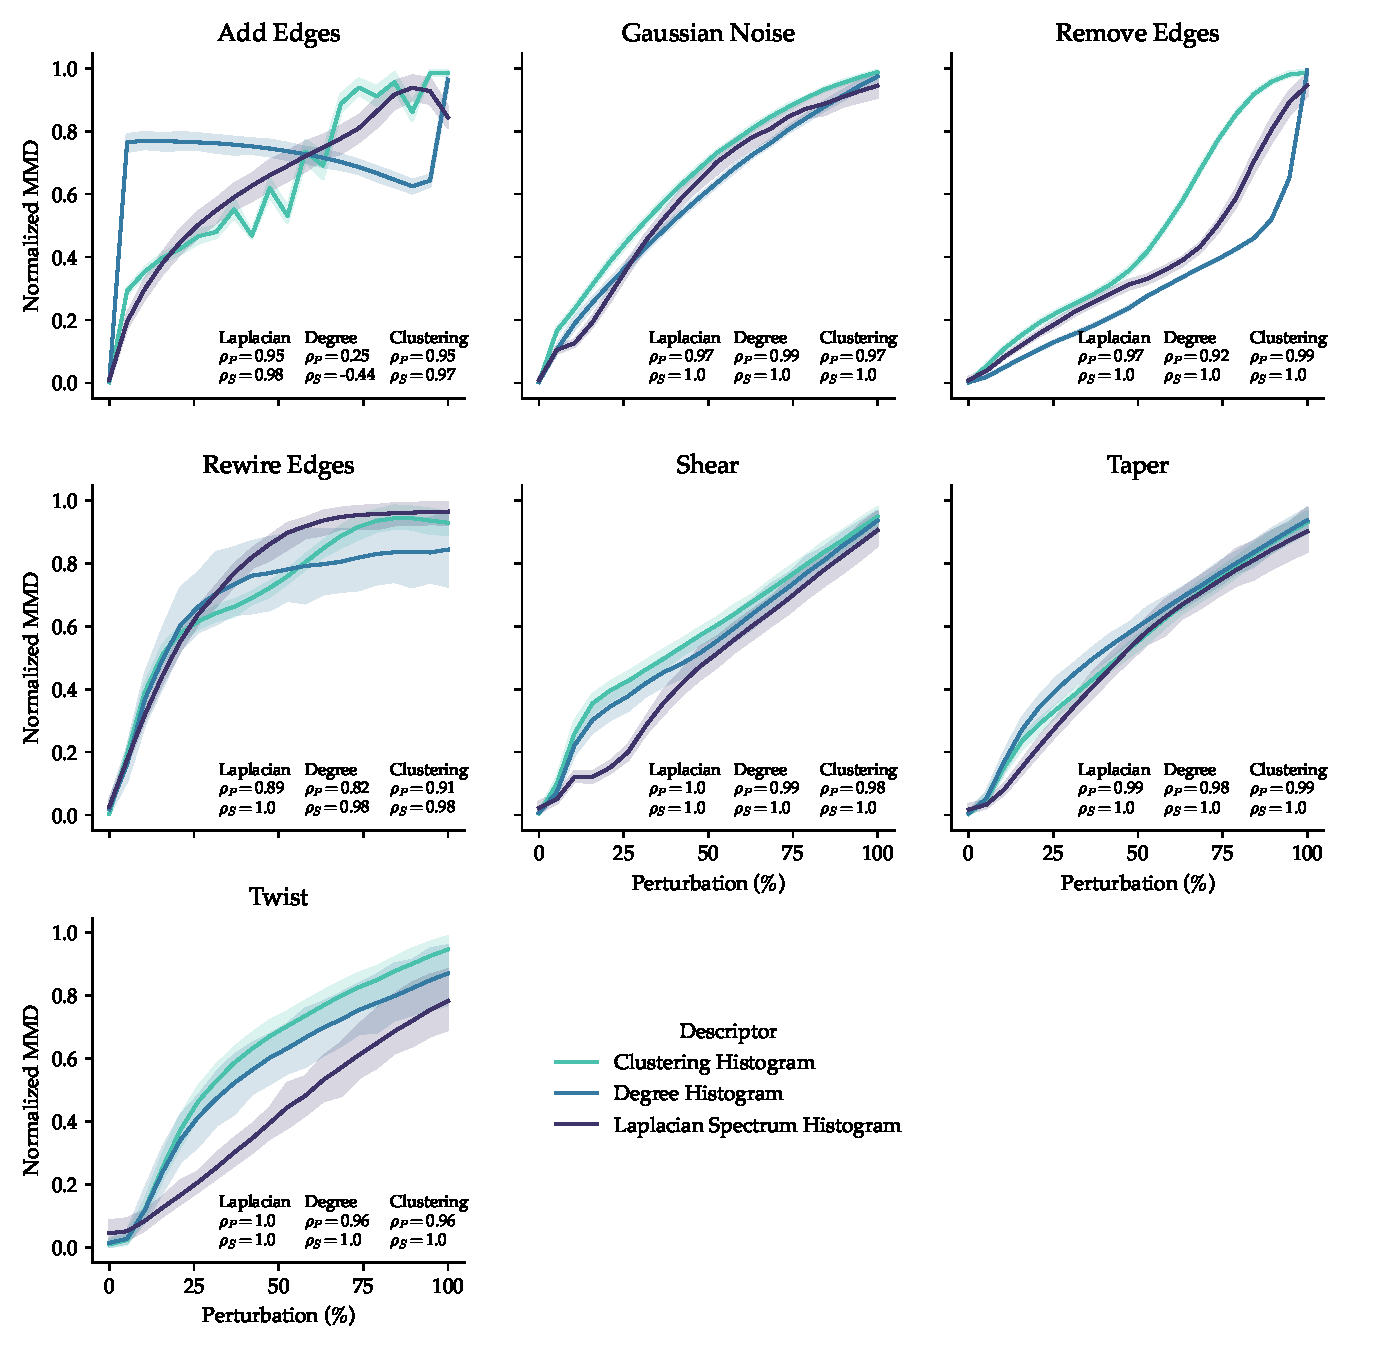
\includegraphics[width=\textwidth]{./figures/results/res_1_1.pdf}
  \caption[Overall behaviour of \acrshort{mmd} using graph-based descriptors.]{\acrshort{mmd} vs.
perturbation (in \%) for various graph descriptors of the 8\si{\angstrom}-graphs
under different perturbations regimes. The kernel used to obtain these graphs is
the RBF Kernel with bandwidth 0.01. $\rho_{S}$: average Spearman correlation
coefficient across runs. $\rho_{P}$: average Pearson correlation coefficient
across runs. Save for the degree histogram behaviour when edges are added, we
see that most \acrshort{mmd} configurations behave well, i.e. there is a high correlation
betweeen the \acrshort{mmd} values and the perturbation.}
  \label{fig:mmd_consistent_eps}
\end{figure}


\begin{figure}
  \centering
  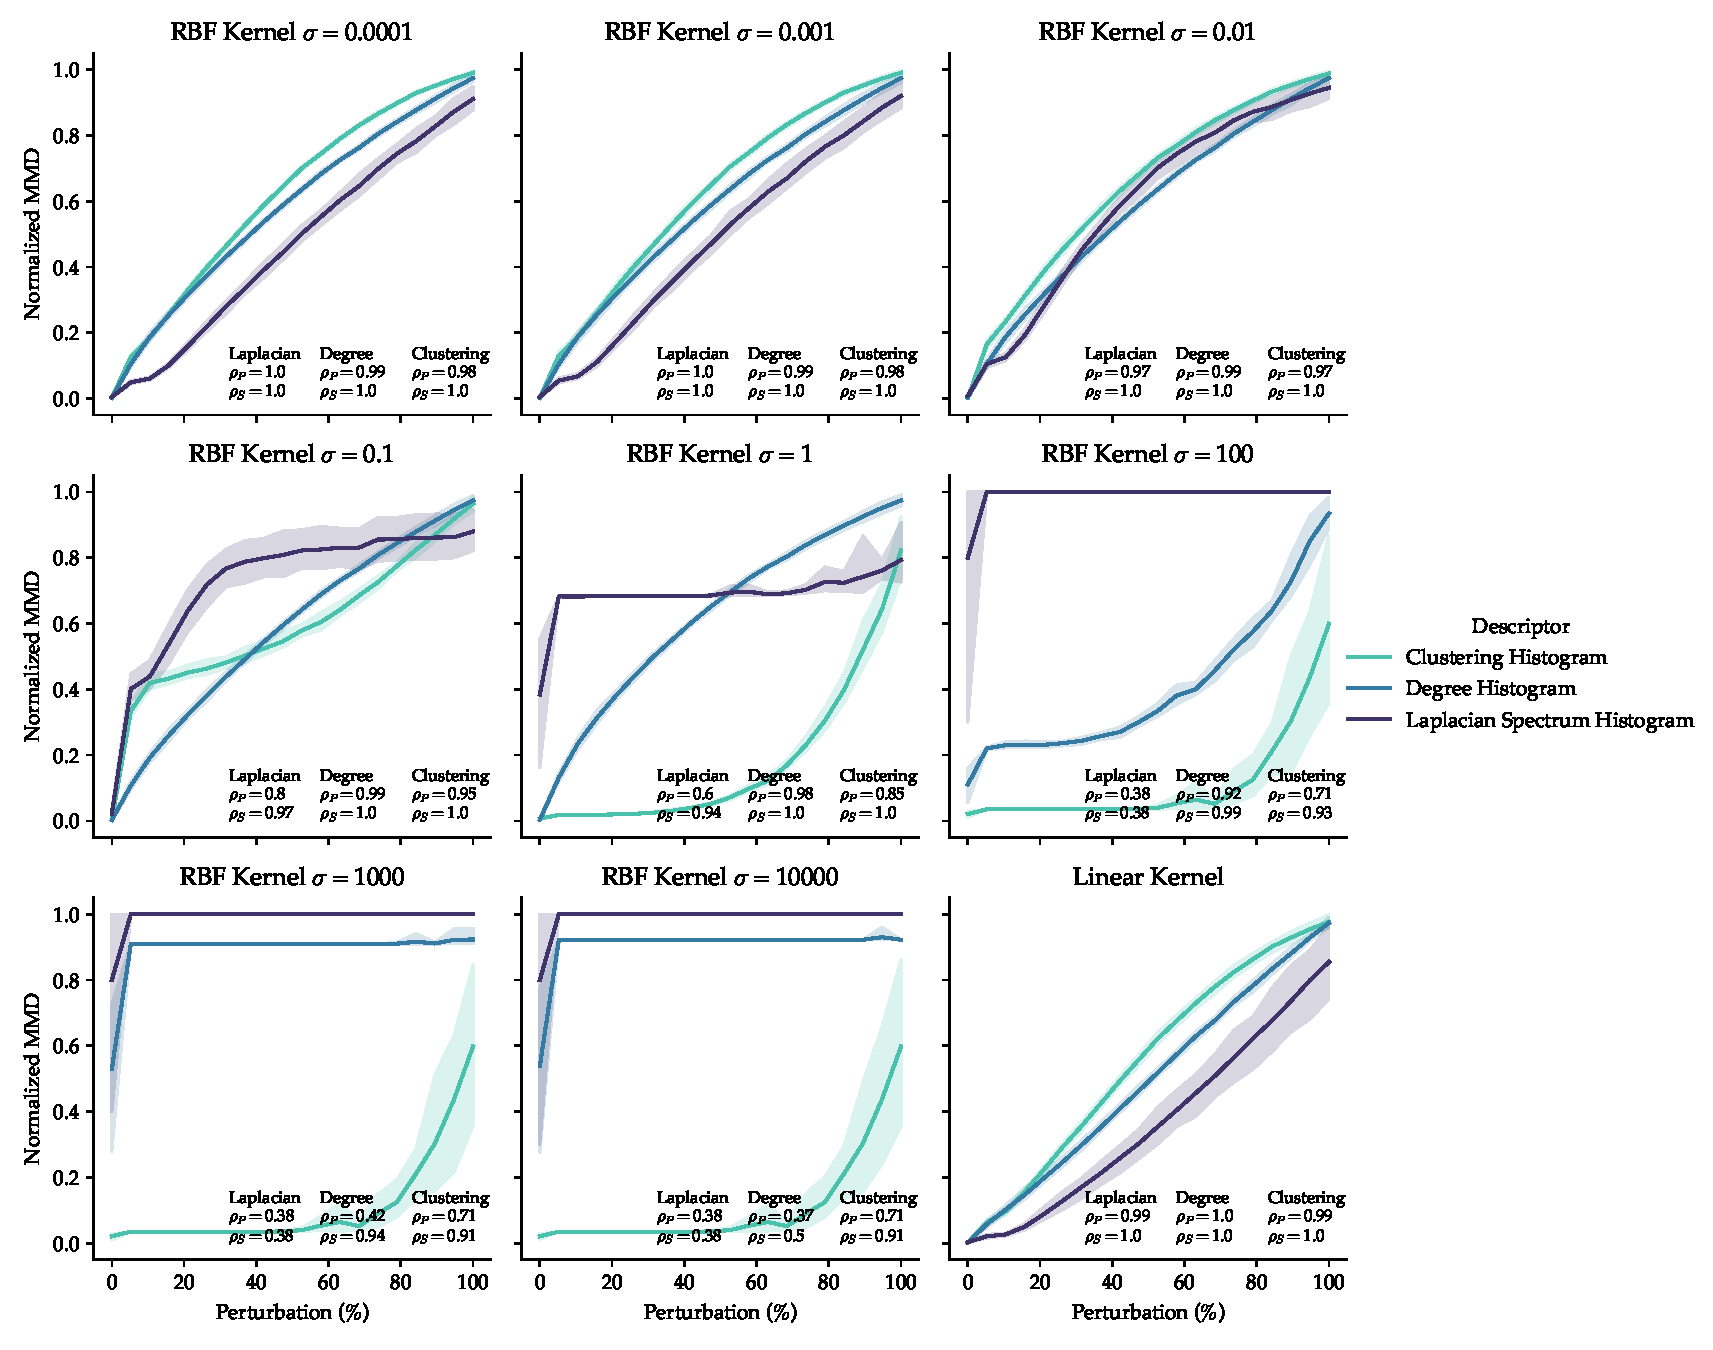
\includegraphics[width=\textwidth]{./figures/results/res_1_2.pdf}
  \caption[Influence of kernel parameters on \acrshort{mmd} behaviour.]{\acrshort{mmd} vs. Gaussian
noise perturbation (in \%) for various graph descriptors of the
8\si{\angstrom}-graphs. $\rho_{S}$: average Spearman correlation coefficient
across runs. $\rho_{P}$: average Pearson correlation coefficient across runs.
The kernel here is shown on top of each subplots. We can see that reasonable
behaviour of the RBF kernel can be seen when $\sigma<1$. The linear kernel also
behaves well.}
  \label{fig:mmd_effect_kernel}
\end{figure}

\begin{figure}
  \centering
  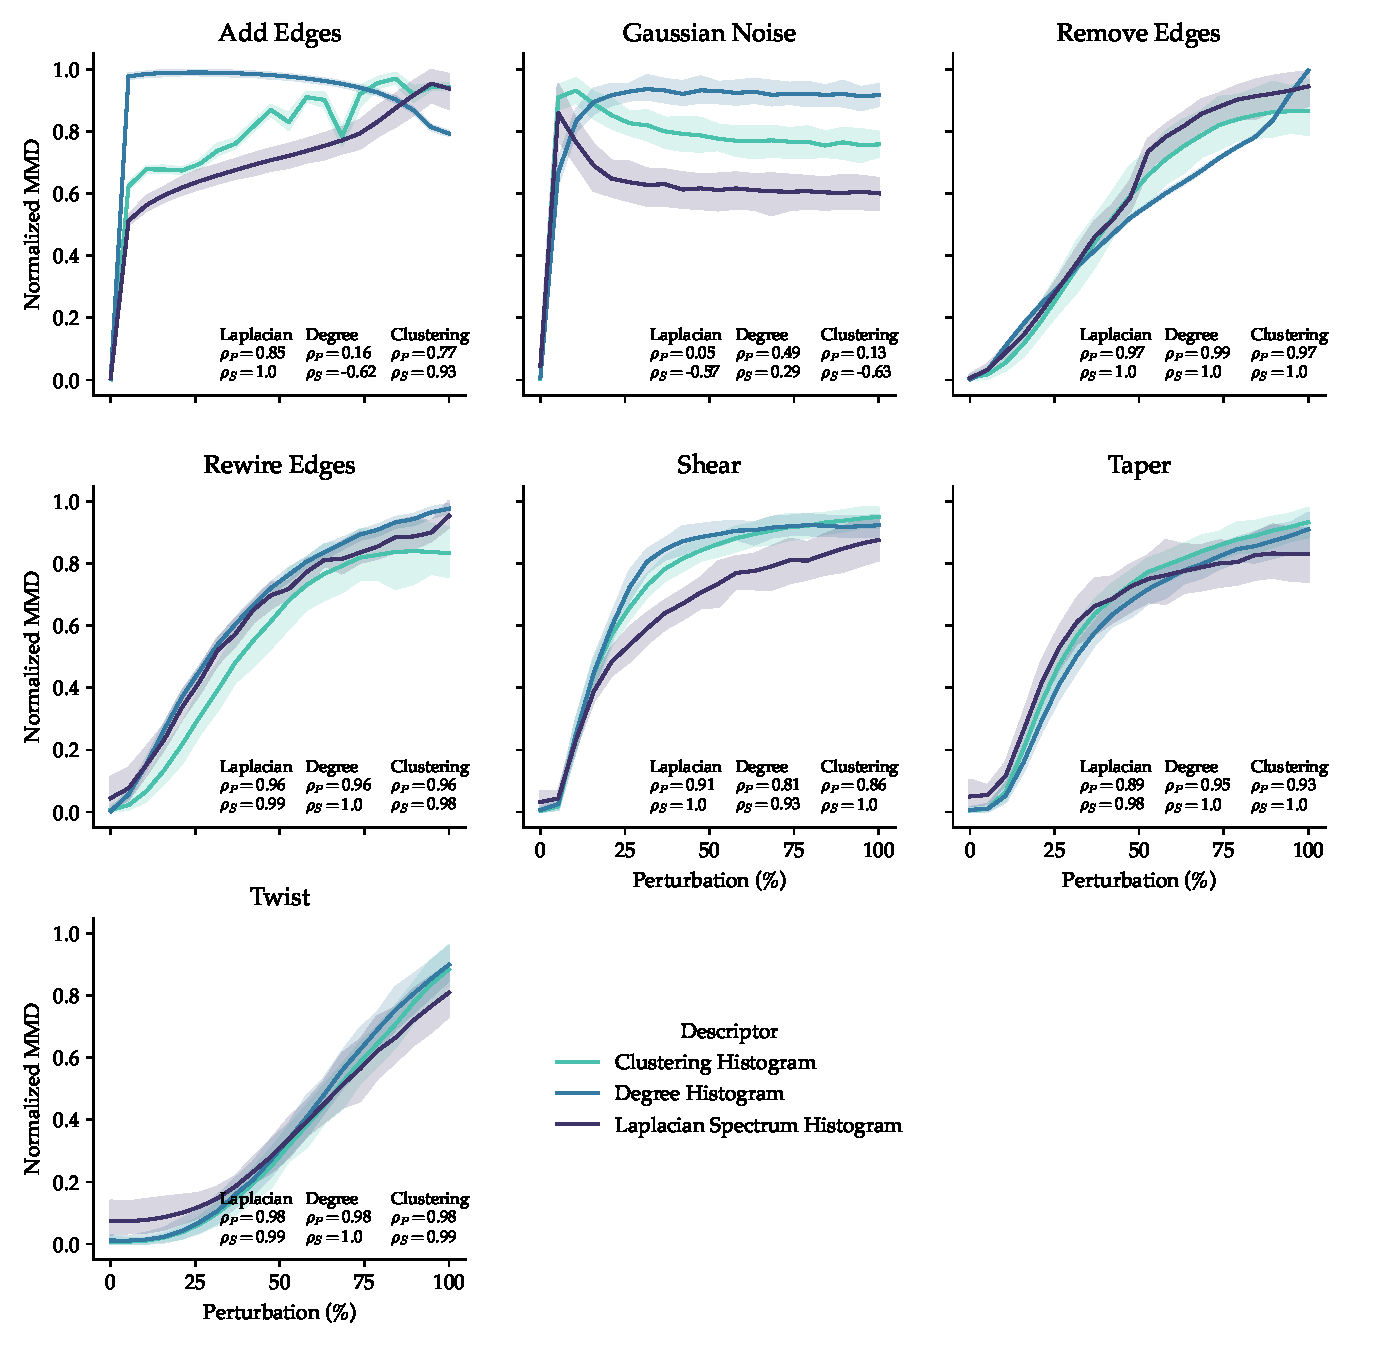
\includegraphics[width=\textwidth]{./figures/results/res_1_3.pdf}
  \caption[2-nearest-neighbour graphs result in descriptors highly sensitive to
the addition of edges and Gaussian noise.]{\acrshort{mmd} vs. Gaussian noise perturbation
(in \%) for various graph descriptors of the 2-nearest-neighbour graphs.
$\rho_{S}$: average Spearman correlation coefficient across runs. $\rho_{P}$:
average Pearson correlation coefficient across runs. We can see that this
particular representation results in \acrshort{mmd} values that are very sensitive to the
addition of edges or Gaussian noise, regardless of the descriptor used.}
  \label{fig:mmd_k_nn_graphs}
\end{figure}

\begin{figure}
  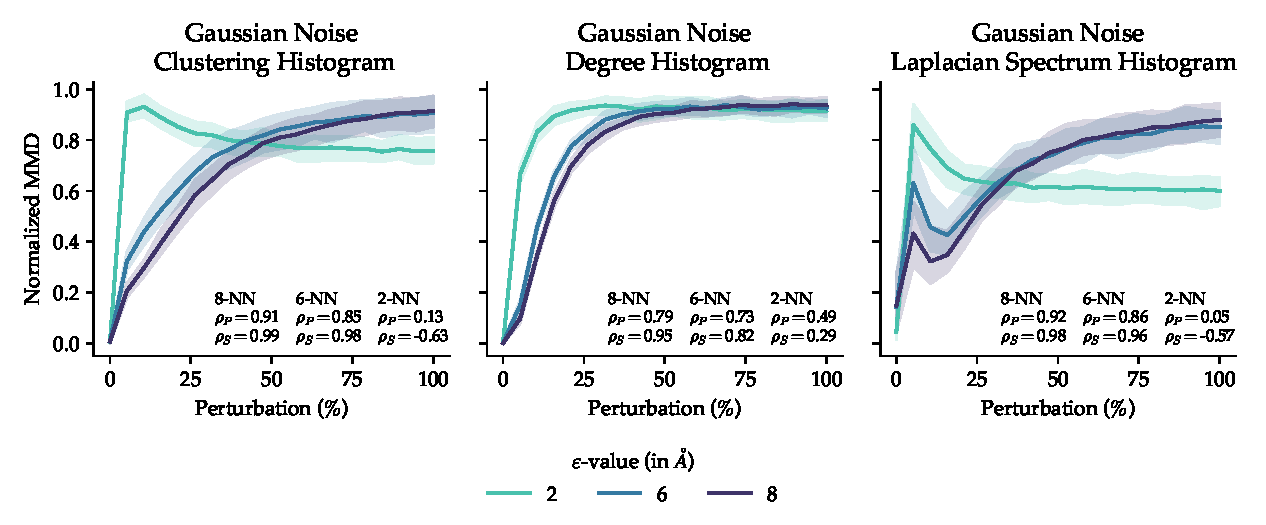
\includegraphics[width=\textwidth]{./figures/results/res_1_4.pdf}
  \caption[Influence of $k$ on the resulting \acrshort{mmd} values.]{\acrshort{mmd} vs. Gaussian noise
perturbation (in \%) for various graph descriptors and values of $k$ used to
extract the $k$-NN graph. $\rho_{S}$: average Spearman correlation
coefficient across runs. $\rho_{P}$: average Pearson correlation coefficient
across runs. Overall, the smaller the $k$, the more sensitive the
\acrshort{mmd}. Choosing $k=2$ results in sometimes unpredictable behaviour depending on
the descriptor chosen (like the clustering and laplacian spectrum histograms).}
  \label{fig:k_vs_turbulence_gaussian_noise}

\end{figure}

% \acrshort{mmd} is quite stable, somewhat contradicts what obray is saying. Maybe due to
% the different nature of the graphs.

\section{Influence of the graph representation on the sensitivity to perturbations}\label{sec:results_sensitivity}

In the last section, we discussed the notion of sensitivity of a particular \acrshort{mmd}
configuration to perturbations. We explore this idea further here. Specifically,
we investigate the impact of the $\varepsilon$ threshold on the resulting
sensitivity of the \acrshort{mmd} configuration to various perturbations affecting the
underlying point cloud. Figure \ref{fig:mmd_sensitivity_eps} shows that, in
general, the lower the $\varepsilon$, the more sensitive the \acrshort{mmd} to
perturbations. Low sensitivity to perturbation might be useful in the early
stages of modeling when generated samples only need to \emph{coarsely} match
the reference samples. Conversely, a higher sensitivity to perturbations might
be useful when trying to \emph{finely} distinguish a set of anomalous samples
from the reference samples. Additionally, we can see that under the Gaussian
noise, twisting and tapering perturbation, larger values of $\varepsilon$
introduce larger variations in \acrshort{mmd} values.

\begin{figure}
  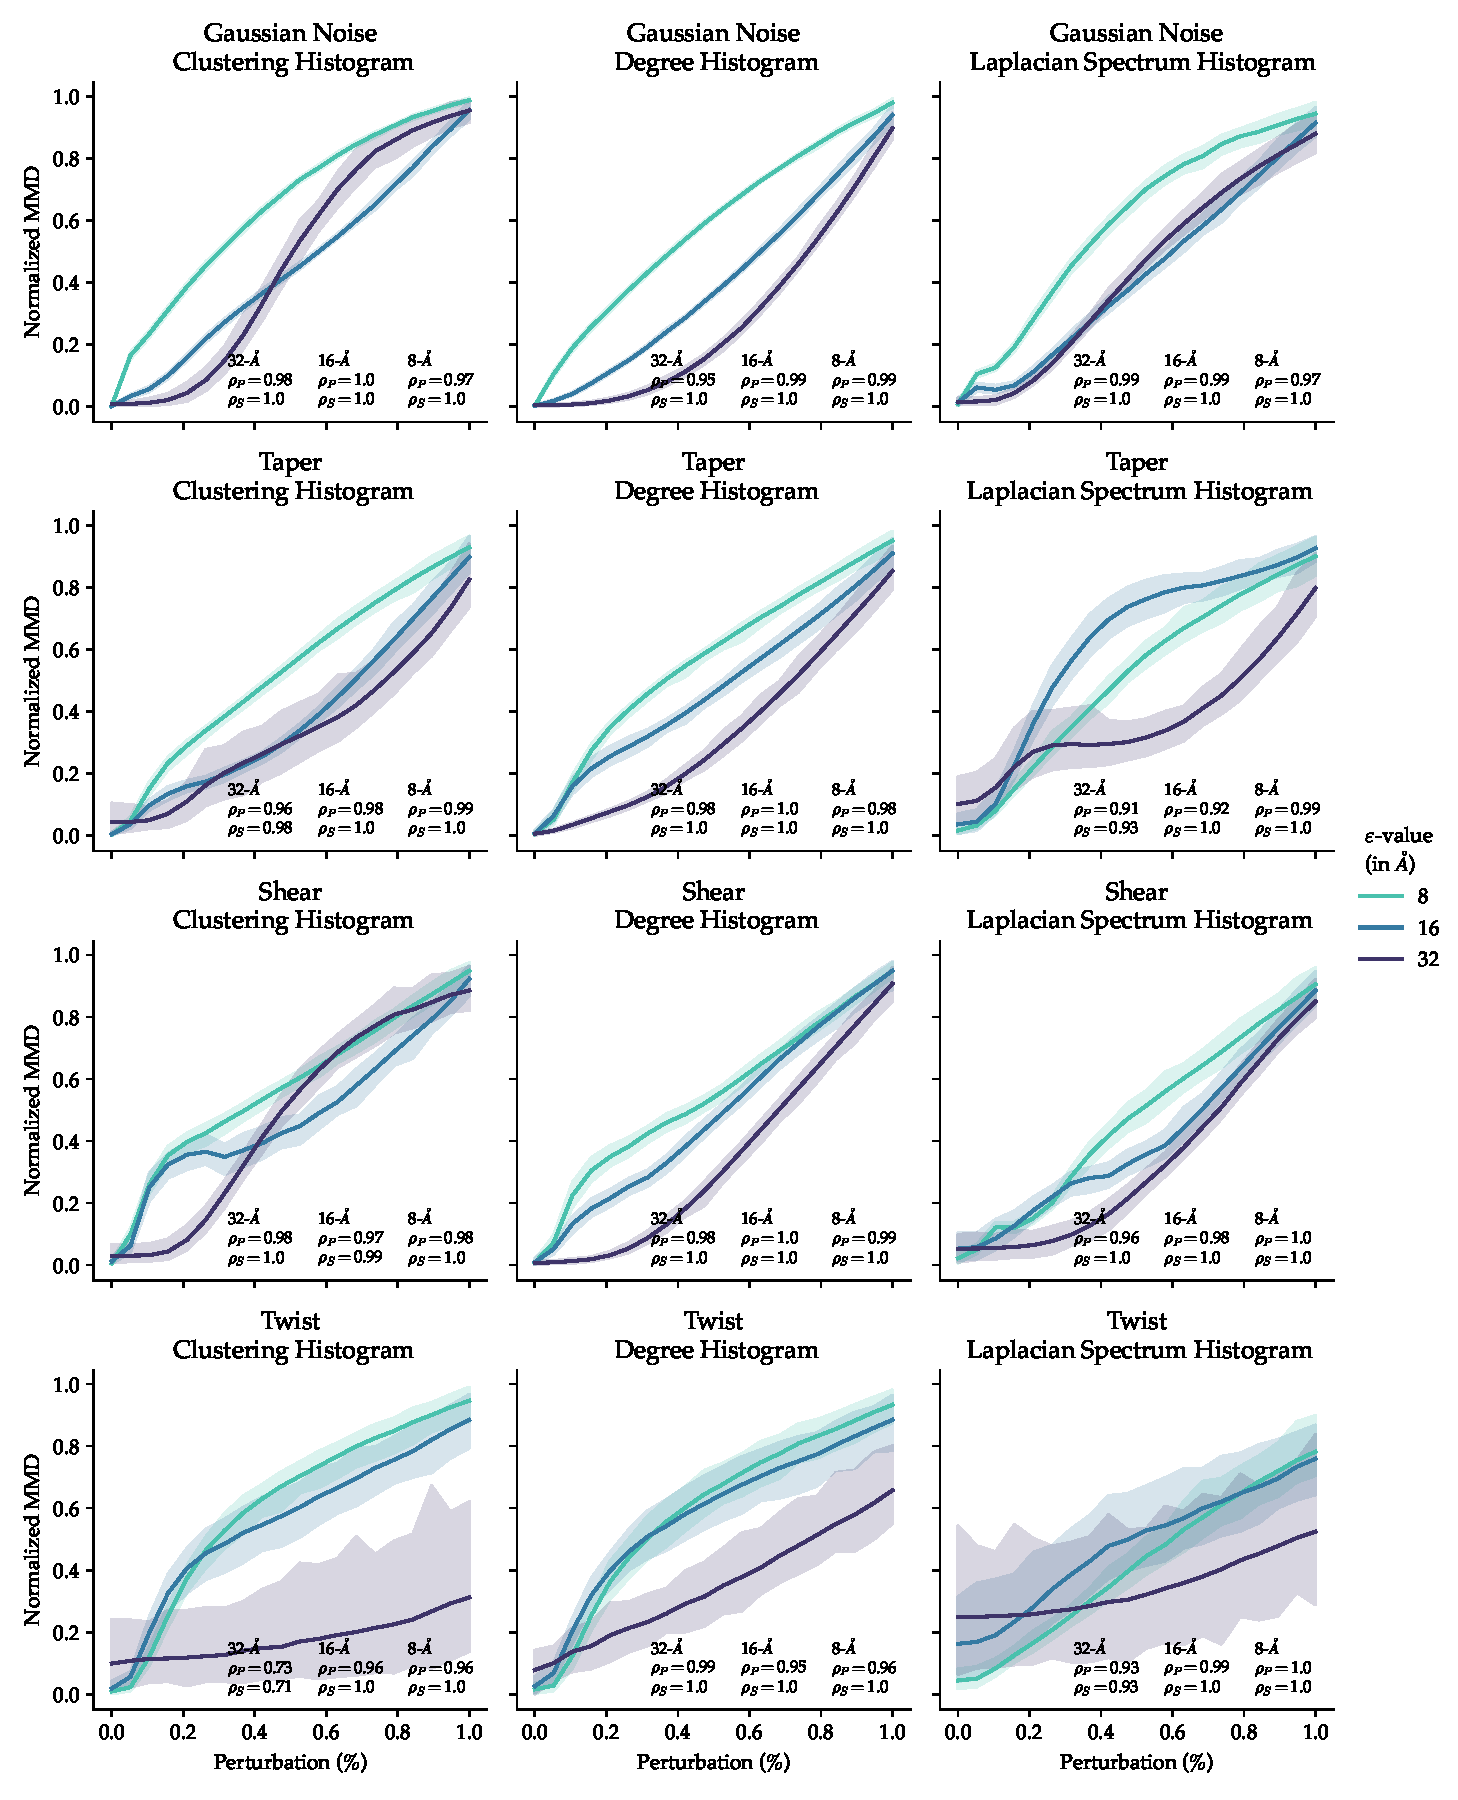
\includegraphics[width=\textwidth]{./figures/results/res_2_1.pdf}
  \caption[Influence of $\varepsilon$ on the sensitivity of \acrshort{mmd} to perturbations.]{\acrshort{mmd} vs. point cloud perturbation for various descriptors. In general,
when graphs are extracted with a lower $\varepsilon$ value, the \acrshort{mmd} curve
increases more rapidly. The only exception to this trend is the laplacian
spectrum histogram descriptor under the tapering perturbation.}
  \label{fig:mmd_sensitivity_eps}
\end{figure}

\section{Graph Kernels}\label{sec:results_graph_kernels}
% TODO compare WL with ESM (no modelling bias for WL on paper, might be a
% weakness since some mutations might not have a functional effect.)

The results of the behavior of the Weisfeiler-Lehman kernel (see Sections
\ref{sec:kernels} and \ref{sec:methods_kernels}) can be seen in Figure
\ref{fig:wlk}. Contrary to the tendencies observed in Section
\ref{sec:results_sensitivity}, \acrshort{mmd}s obtained using the Weisfeiler-Lehmann
kernels on 8\si{\angstrom} graphs are very insensitive to medium levels of perturbations,
and even completely oblivious to rewiring of graphs and generally insensitive to
graph perturbations unless highly perturbed (see upper row of Figure \ref{fig:wlk}). The most likely explanation
is that the diversity of Weisfeiler-Lehman hashes (i.e. neighborhoods) observed within perturbed or
unperturbed samples is relatively high, which makes distinguishing between the
two a high threshold to overcome. This drawback could disappear if one is working on
a more targeted set of morphologically similar proteins with a lower diversity
of Weisfeiler-Lehman hashes, but this is beyond the scope of the thesis.

\begin{figure}
  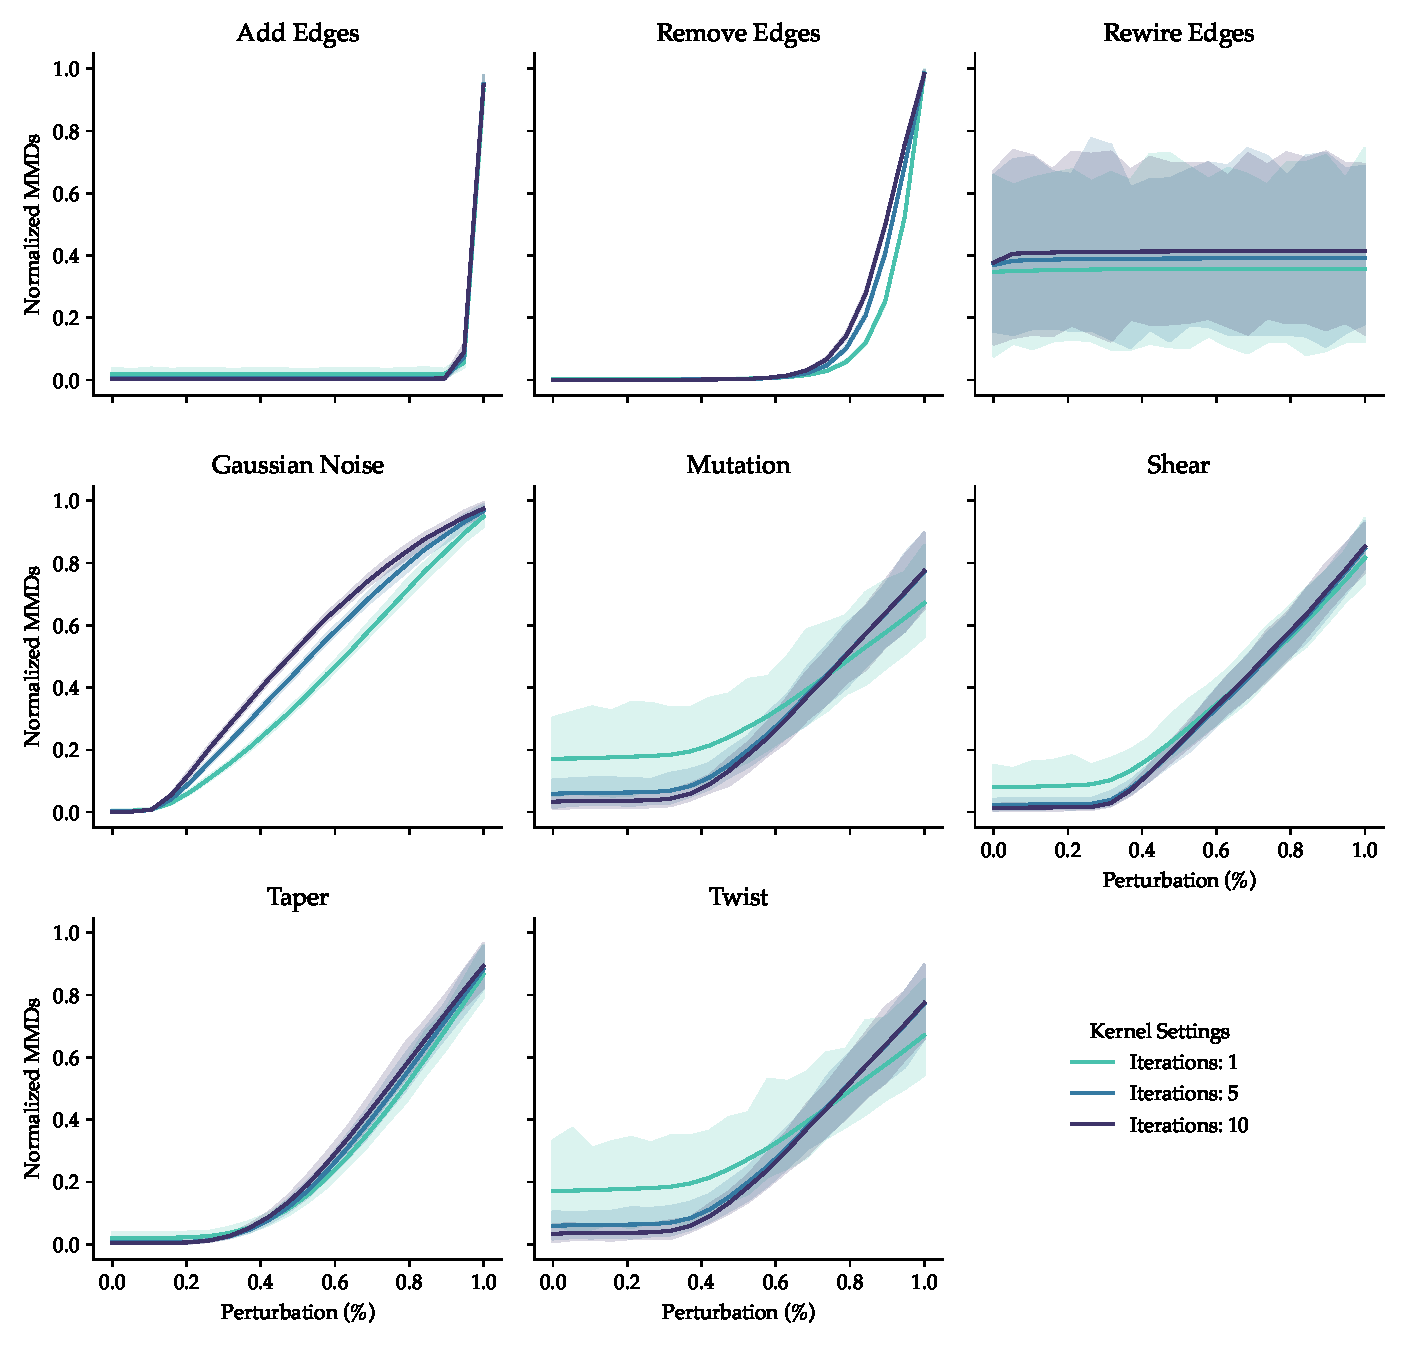
\includegraphics[width=\textwidth]{./figures/results/res_3.pdf}
  \caption[Normalized \acrshort{mmd} values using the Weisfeiler-Lehman kernel subject to
  various perturbations.]{\acrshort{mmd} vs.
perturbations using the Weisfeiler-Lehman kernel using the
8\si{\angstrom}-graphs as inputs. We see that high levels of perturbations are
required to raise the normalized \acrshort{mmd} values. We also see that \acrshort{mmd}s computed with
the Weisfeiler-Lehman kernel are insensitive to the rewiring of edges, and
results in \acrshort{mmd}s with a high inter-run variance.}
  \label{fig:wlk}
\end{figure}

\section{Protein-specific descriptors}\label{sec:results_protein_descriptors}

The behaviour of \acrshort{mmd} values derived from the protein-specific descriptor
functions described in section \ref{sec:descriptors} are shown in Figure
\ref{fig:protein_specific_descriptors}. The dihedral angles descriptor is
extremely sensitive to any kind of Gaussian noise and even decreases in value
when the kernel is not parametrized properly when increasing the shearing. This
is overall a good sign, as it will flag proteins that are unrealistic. The
interatomic distance histogram also behaves well. However, it shows high
variance when twisting the protein, presumably because the intra-sample variance
in distances is a threshold hard to overcome. This phenomenon can also be
noticed in Figure \ref{fig:wlk} with the Weisfeiler-Lehman kernel and could
disappear when working on morphologically similar proteins as highlighted in
Section \ref{sec:results_graph_kernels}. Another attractive aspect of this class
of descriptors is that they are very cheap to compute -- see further results in
Section \ref{sec:results_runtime}.

\begin{figure}
  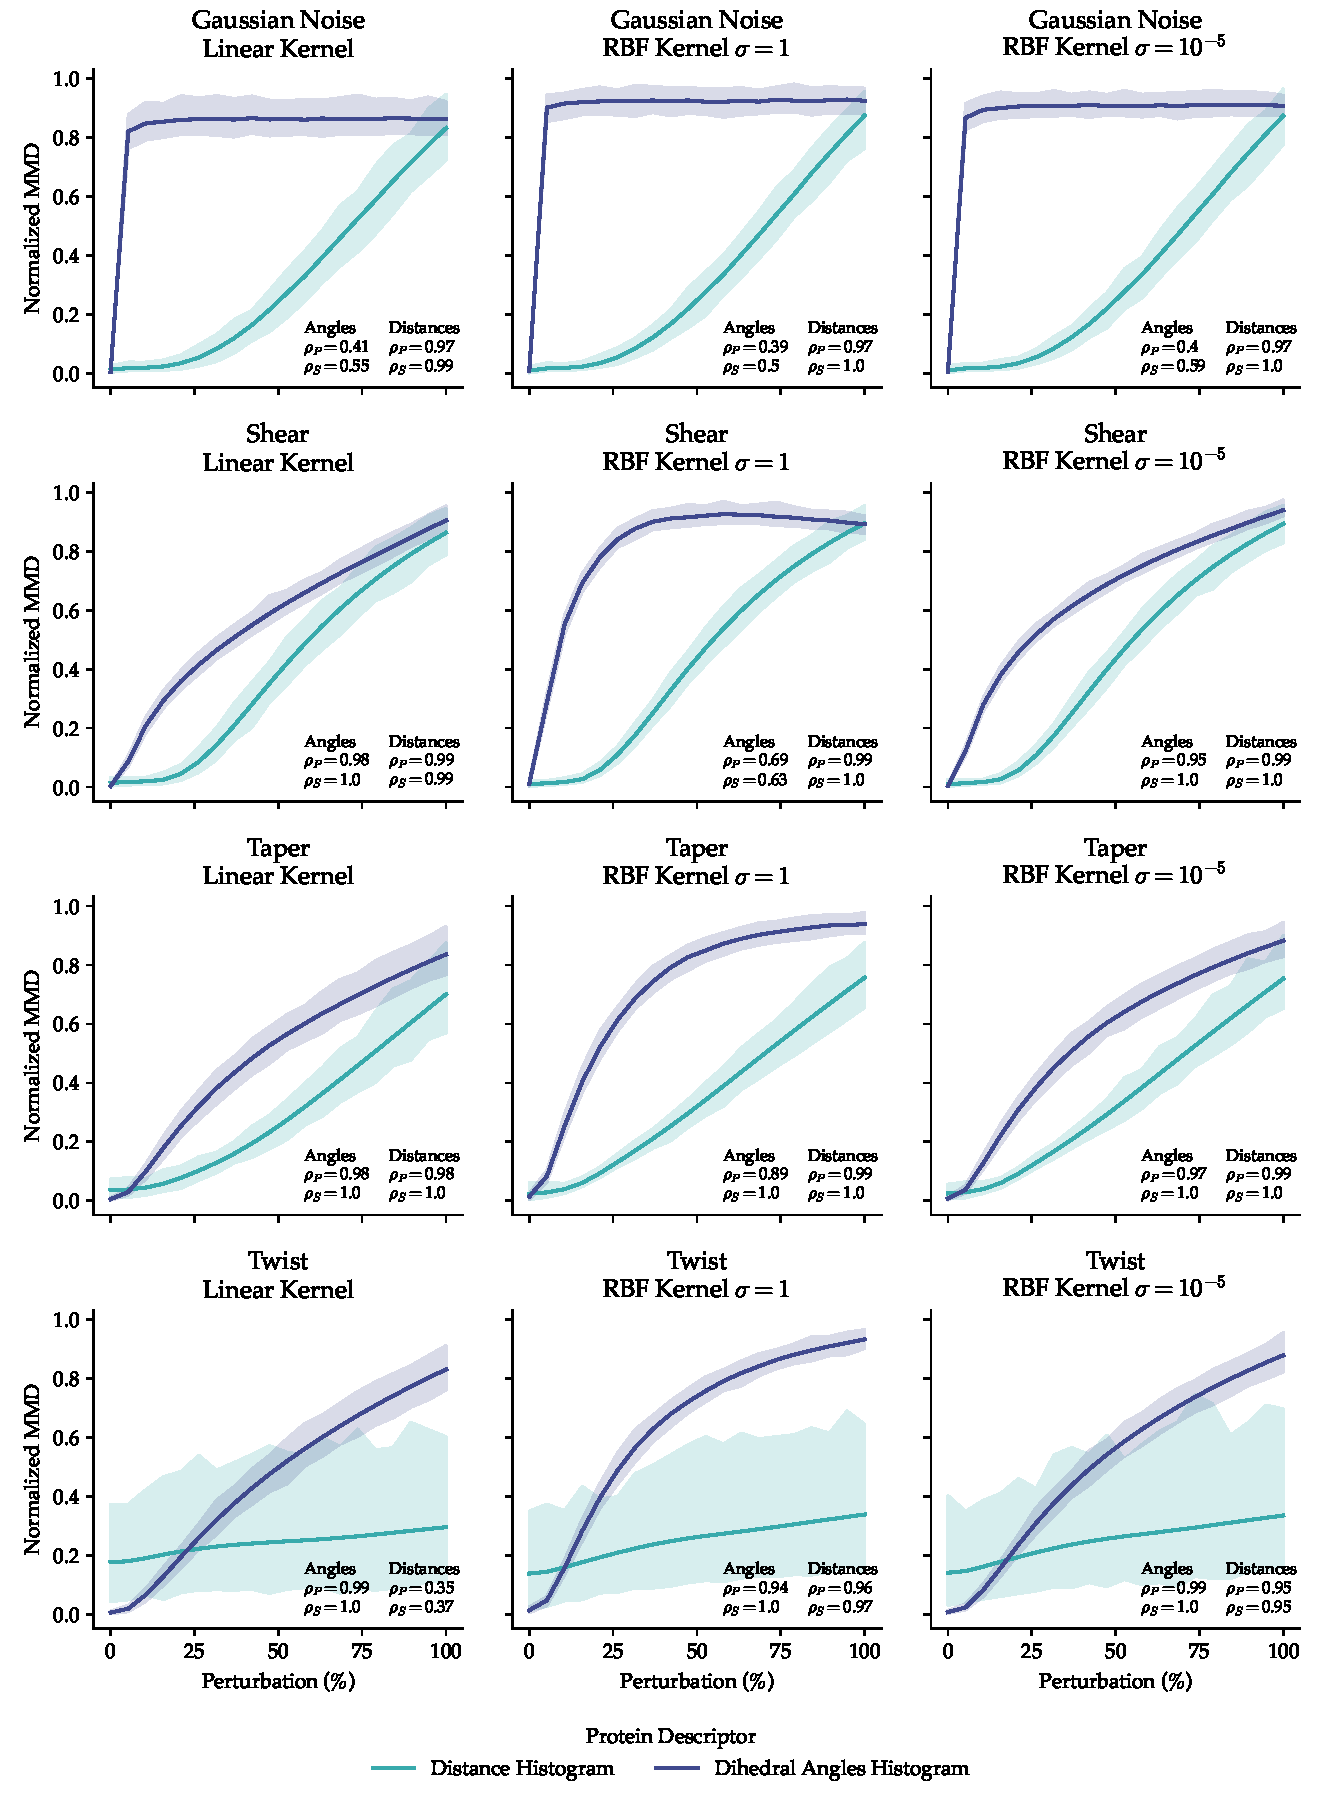
\includegraphics[width=\textwidth]{./figures/results/res_4.pdf}
  \caption[\acrshort{mmd} vs. perturbations using the two novel protein descriptors.]{\acrshort{mmd}
vs. perturbations (in \%) using the two novel protein descriptors shown in Section
\ref{sec:descriptors}. Various kernel configurations are shown here. Those
descriptors behave very well overall, with the dihedral angles descriptors being
especially sensitive to Gaussian noise. The distance histogram exhibits
particularly higher inter-run variance especially when subject to twisting
pertubations.}
  \label{fig:protein_specific_descriptors}
\end{figure}

\section{\acrshort{mmd} From Learned Embeddings}

Because the only constraint of the input vectors to the kernels accepting
fixed-length vectors as inputs is that they are in $\R^d$, we can input
fixed-length vector embeddings into them, leveraging the immense progress made
in the past decade regarding embeddings of structured data, specifically protein
sequences as highlighted in Section \ref{sec:mmd}. The only perturbation such a
learned embedding would be sensitive to is changes in the protein sequence. As
such, we investigated how the \acrshort{mmd} values increase with increasing point mutation
probabilities with various kernels, as seen in Figure \ref{fig:esm_descriptor}.
We find that the kernel used does not have any bearing on the \acrshort{mmd} behavior as
long as $\sigma<1$ for the RBF kernel. Overall, we see that even in these low
mutation regimes, the \acrshort{esm} embedding is sensitive enough to detect such changes.
More sequence-specific perturbations are required to assess the
applicability of the \acrshort{esm} embedding as a sequence descriptor, such as
translocation of subsequences, additions, deletions, etc. However, the early
results of such a descriptor shown in this thesis are promising

\begin{figure}
  \centering
  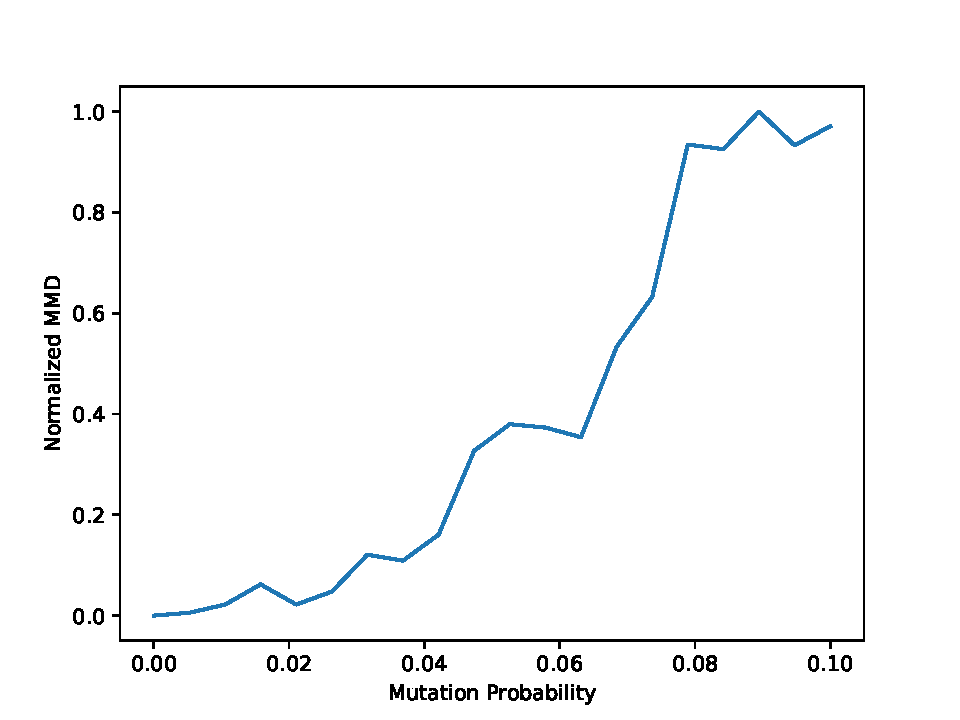
\includegraphics[width=\textwidth]{./figures/results/res_5.pdf}
  \caption[\acrshort{mmd} using \acrshort{esm} embeddings.]{\acrshort{mmd} vs. mutation probability using the \acrshort{esm}
learned embeddings with various kernels. The correlation coefficients of the
resulting \acrshort{mmd}s with RBF kernels with $\sigma<1$ and the linear kernel are high,
therefore making them good configurations for sequences. This analysis should be
complemented by complementary sequence-specific perturbations -- see Section
\ref{sec:discussion_realistic_proteins} for details.}
  \label{fig:esm_descriptor}
\end{figure}


\section{Topological Descriptors And Kernels}\label{sec:results_topo_kernels}

Figure \ref{fig:tda_kernels} shows the behavior of both the multi-scale kernel
and persistence Fisher kernel. Overall, we can see that they are among the best
performing metrics in this thesis, with high correlations and low inter-run
variation. While they cannot detect changes in node labels in the current
setting, hence not being able to detect mutations, we will show in Section
\ref{sec:tda_limitations} how this could be alleviated. For computational
reasons, we did not compute variations of different kernel parameters, although
one could speed up the operation by precomputing the kernel matrices, and only
later multiplying the matrix by different constants (see Appendix A.5 of
\cite{o2021evaluation}).

\begin{figure}
  \centering
  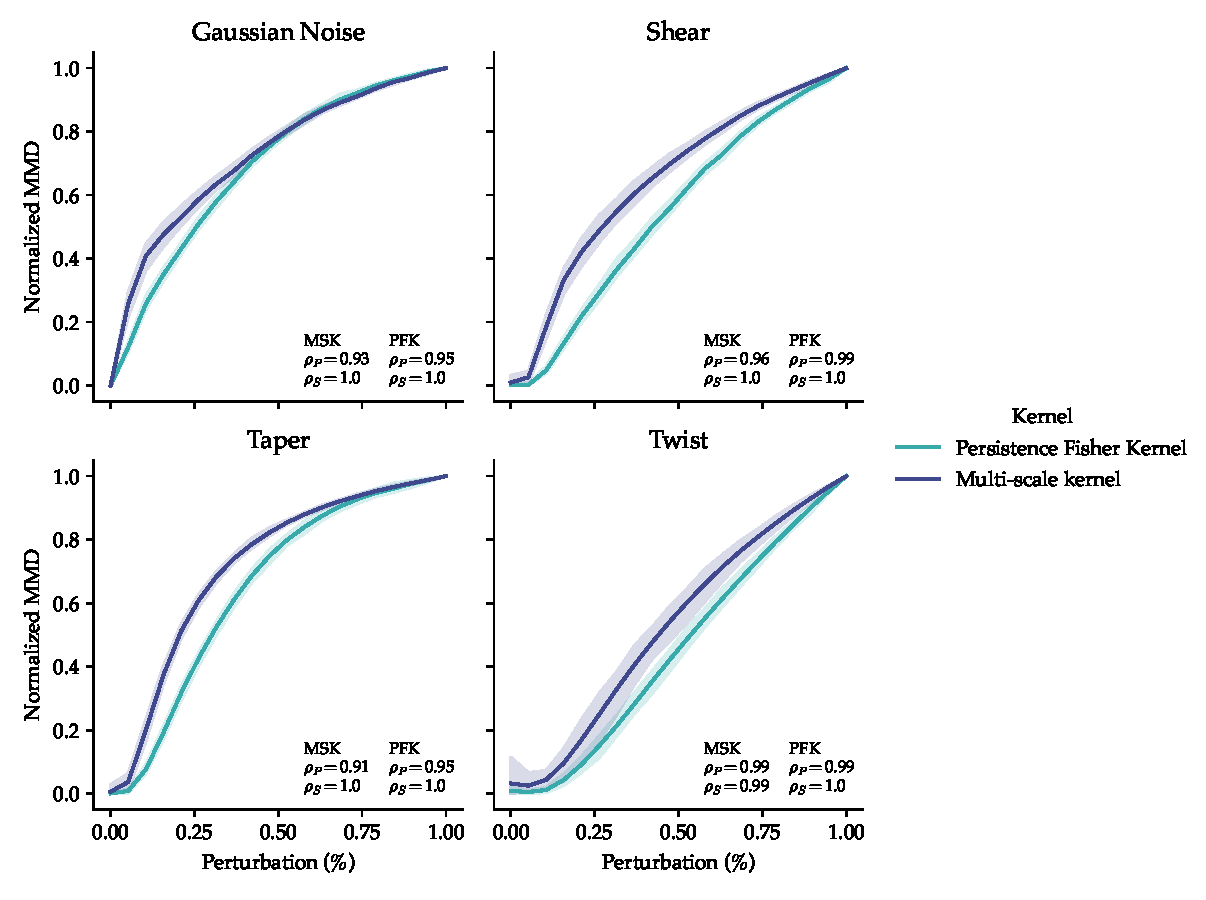
\includegraphics[width=\textwidth]{./figures/results/res_6.pdf}
  \caption[\acrshort{mmd} using topological kernels.]{\acrshort{mmd} vs. Perturbation (in \%) using the multi-scale
kernel and persistence Fisher kernel. For the persistence Fisher kernel, both
the kernel bandwidth parameter and the Fisher bandwidth parameter are set to 1.
For the multi-scale kernel, the bandwidth parameter is also set to 1. Overall,
the correlation coefficients for those kernels are very high and show little
inter-run variance.}
  \label{fig:tda_kernels}
\end{figure}


\section{Variance}

In Figures \ref{fig:mmd_consistent_eps} through \ref{fig:tda_kernels}, we mostly
commented on the correlation coefficients between the (normalized) \acrshort{mmd} values
and the amount perturbation applied. While a high correlation is certainly a
good indicator of a particular \acrshort{mmd} configuration, one should also carefully
consider the (normalized) inter-run variance observed between independent
samples of proteins. We can see that in Figures \ref{fig:mmd_consistent_eps}
through \ref{fig:tda_kernels}, this variance changes quite a lot depending on
the \acrshort{mmd} configuration. It can be especially high for certain representations.
For instance in Figure \ref{fig:mmd_sensitivity_eps}, one can see that a higher
$\varepsilon$ value (e.g. 32\si{\angstrom}) show a higher inter-run variance
compared to a lower $\varepsilon$ value (e.g. 8\si{\angstrom}), especially when
it comes to the twisting perturbation (lowest row). Furthermore, one of the
descriptors devised for this thesis also exhibits high variance under twisting
perturbations: the pairwise distance histogram, Figure
\ref{fig:protein_specific_descriptors}. The consequence of a high normalized
inter-run variance can be just as nefarious as \acrshort{mmd} configurations with low
correlation coefficients because the range of absolute \acrshort{mmd} values can be too wide
to make an accurate assessment of the quality of generated samples.


\section{Runtime}\label{sec:results_runtime}

One of the desiderata of \acrshort{mmd} is a low computational complexity (see Section
\ref{sec:evalproblem}). As such, we report the various computation times for
each of the important elements of the pipelines outlined in this thesis. The
summary of all execution times can be found in Table \ref{tab:runtimes}.

First, we see that one computation stands out: computing the Vietoris-Rips
filtration of a point cloud. Together with a large memory footprint, the
Vietoris-Rips filtration is quite lengthy to compute, due to a runtime of
$\mathcal{O}(n^{3(k+2)})$, where $k$ is the number of dimensions (here, $k=3$)
and $n$ the number of points \citep{adams2018persistent}. Although some optimizations have been carried out
by \texttt{Ripser}, the software used to compute the Vietoris-Rips filtration,
it remains very expensive to compute and does not enjoy the benefits of hardware
acceleration through e.g. a GPU due to the difficulty of parallelizing such a
filtration \citep{Bauer2021Ripser}.

Second, computing the distance histogram and dihedral angles histogram is the
fastest descriptors to compute, making them suitable to evaluate large
collections of generated proteins. Other graph descriptors are also reasonably
fast to compute, but they depend on the settings used to extract the graphs, and
generally, the runtime increases in the number of edges of the graph.

Third, the kernels used in this study all have reasonable runtimes, but we note
the particular efficiency of the RBF and linear kernel compared to the
persistence Fisher, multi-scale and Weisfeiler-Lehmann kernel. The
implications of these runtimes will be further explored when making
recommendations to the practioner in Section
\ref{sec:discussion_recommendations}.


\begin{table}
  \centering
  \begin{tabular}{lll}
    \toprule
    \textbf{Operation} &  \textbf{Execution Time} \\
    \midrule
    \textbf{Descriptor Functions} & \\
    \midrule
    Vietoris-Rips Filtration & 3332 s \\
    \acrshort{esm} Embedding & 163 s\\
    Degree Distribution Histogram (32\si{\angstrom}-graph) & 35 s\\
    Clustering Coefficient Histogram (32\si{\angstrom}-graph) & 175 s\\
    Laplacian Spectrum Histogram (32\si{\angstrom}-graph) & 35 s\\
    Distance Histogram & 28 s\\
    Dihedral Angles Histogram & 4 s\\
    \midrule
    \textbf{Kernels} & \\
    \midrule
    Weisfeiler-Lehman Kernel (4 iterations) & 32 s \\
    Persistence Fisher Kernel & 35 s \\
    Multi-Scale Kernel & 11 s \\
    RBF Kernel  & 1.7 ms \\
    Linear Kernel  & 7.7 ms \\
    \bottomrule
  \end{tabular}
  \caption[Runtime and computational complexity of the various elements of the
  pipeline.]{Runtime and computational complexity of the various elements of the
pipeline. These timings are obtained by executing the operation on 100 samples
spread across 10 CPU cores from an Intel Xeon Gold 6254 CPU clocked at 3.10GHz.}
  \label{tab:runtimes}
\end{table}


\section{Summary}

In this chapter, we present the results of the behavior of \acrshort{mmd} under various
configurations and subject to various perturbations. We first note that the
overall behavior of \acrshort{mmd} under various perturbations is stable when sufficient
care is put into the selection of the of the kernel parameters (Figure \ref{fig:mmd_consistent_eps}). As a side note,
we see also that overall the correlations for descriptors of
$\varepsilon$-graphs is better than for $k$-NN graphs (Figure \ref{fig:mmd_k_nn_graphs}). Second, we note that the
choice of graph representation impacts the behavior of \acrshort{mmd}'s behavior: the
lower the radius of the sphere used to extract the $\varepsilon$-graph, the more
sensitive the resulting \acrshort{mmd} configuration, i.e. the lower the perturbation
required for the \acrshort{mmd} to reach a certain threshold (Figure
\ref{fig:mmd_sensitivity_eps}).

We then present the results for more exotic configurations of \acrshort{mmd} which we
hypothesized might be uniquely suited for protein representations. First, we
investigate the applicability of graph kernels, specifically the
Weisfeiler-Lehman kernel, to graphs extracted from proteins, which revealed that
high levels of perturbations are required to detect changes in \acrshort{mmd} (Figure
\ref{fig:wlk}). We then presented the results of the efficient and biologically
relevant protein-specific descriptors, which seem to behave very well (Figure
\ref{fig:protein_specific_descriptors}). Using learned embeddings as sequence
descriptors such as the \acrshort{esm} embedding showed that the resulting \acrshort{mmd} is sensitive
to low rates of point mutation (Figure \ref{fig:esm_descriptor}). Using
topological descriptors and appropriate kernels also seems to work very well, despite
a high computational cost (Figure \ref{fig:tda_kernels}). Finally, we show the
results of the runtime of each significant operation of the workflow highlighted
in this thesis (Table \ref{tab:runtimes}).

\chapter{Discussion}\label{chap:discussion}

In this chapter, we discuss the findings of this thesis presented in Chapter
\ref{chap:results}, which we will summarize in Section \ref{sec:key_findings}.

\section{Key Findings}\label{sec:key_findings}

Overall, we found that \acrshort{mmd} behaved surprisingly well on graphs extracted from
proteins (e.g. see Figure \ref{fig:mmd_consistent_eps}). This finding is
somewhat surprising considering recent findings indicating the relative
instability of \acrshort{mmd} on synthetic graphs such as Watts-Strogatz graphs and
Barabási–Albert graphs under some combinations of kernels and descriptors
\citep{o2021evaluation}. While we certainly found unstable configurations
(see for instance Figure \ref{fig:mmd_consistent_eps} upper left pane with the degree histogram),
this was not the rule.

Furthermore, we found that the sensitivity of the \acrshort{mmd} to perturbation was
greatly influenced by the graph representation extracted from the protein.
Namely, for $\varepsilon$ graphs (which overall seemed more stable than $k$-NN
graphs), the higher $\varepsilon$, the lower the sensitivity to low levels of
perturbation (Figure \ref{fig:mmd_sensitivity_eps}).

We introduced in Section \ref{sec:descriptors} and shown in Section
\ref{sec:results_protein_descriptors} two \emph{novel} protein-specific descriptors for
used in \acrshort{mmd}, which are both extremely fast to compute (Table \ref{tab:runtimes})
and are able to detect perturbations with a surprising sensitivity (Figure
\ref{fig:protein_specific_descriptors}).

Furthermore, we found that the Weisfeiler-Lehman kernel, introduced in Section
\ref{sec:methods_kernels}, applied to \acrshort{mmd} was able to detect perturbations
unable to be detected by traditional graph descriptors such as point mutations,
which are relevant for the protein domain (Section
\ref{sec:results_graph_kernels}). However, as with the rest of the perturbations,
the Weisfeiler-Lehman kernel is not sensitive to lower regimes of perturbation
(see Figure \ref{fig:wlk}).
This can be alleviated by using an alternative descriptor such as the ESM
protein embedding introduced in Section \ref{sec:evalproblem}, which is more
sensitive to lower rates of point mutation (see Figure
\ref{fig:esm_descriptor}).

We analyzed the \acrshort{mmd} obtained from kernels operating on persistence diagrams in
Section \ref{sec:results_topo_kernels}, which also seemed very promising since
\acrshort{mmd} values leveraging topological kernels both exhibit high correlations to
point cloud perturbations and low inter-run variance.

\section{Practical Recommendations}\label{sec:discussion_recommendations}

Leveraging those key findings, we now formulate a set of recommendations for a
practitioner who needs to evaluate a generative protein model using one of the
protein representations highlighted above.


\subsection{Setup And Baselines}\label{sec:discussion_baselines}
% p-values, violin plots to visualize mmd.

Overall, we advise the practitioner to carefully evaluate certain baselines when
possible. The first would be to evaluate the \acrshort{mmd} between different
i.i.d. samples of the reference distribution to establish the range of
\acrshort{mmd} to be expected in the best case, which we refer to as the
\emph{positive control}. We conducted such positive control for various MMD
configurations in Appendix \ref{sec:mmd_baselines}. From there, an accurate
assessment of the quality of the model can be made. If the kernel and data
representation allows it, it is also advisable to establish a \emph{negative
control}. This would show the worst possible performance between any two
distributions. Typically, for the biased estimate of \acrshort{mmd}, this value
is $\sqrt{2}$. If this is not possible, as is the case in this thesis (e.g.
there is no negative control for all \acrshort{mmd} values perturbed using the
Gaussian noise), it is useful to examine cases of extreme perturbations and
compare the resulting \acrshort{mmd} values to those. Such an assessment can
provide a surrogate for the negative control and confers a sense of scale for
the particular problem tackled.

Moreover, since the \acrshort{mmd} statistic is the basis for a kernel two-sample test
\citep{gretton2012kernel} (see also Section \ref{sec:mmd}), one can easily
estimate a $p$-value from the statistic between the model's generated
distribution and the empirical distribution.

\subsection{Sensitivity of MMD}\label{sec:discussion_right_mmd}
% Comment also on std dev - could potentially help with the p-value if high.
Depending on the stage of modeling and the coarseness of the desired samples,
one might choose different \acrshort{mmd} configurations. As we have shown in Figure
\ref{fig:mmd_sensitivity_eps} and discussed in Section
\ref{sec:results_sensitivity}, choosing a lower threshold $\varepsilon$ to
extract $\varepsilon$-graphs from a protein point cloud results in a higher
sensitivity to a host of perturbation. In practice, this means that the lower the
$\varepsilon$, the better the \acrshort{mmd} will be at discerning perturbed (i.e.
generated) samples from reference samples. This might be desirable if one needs
highly similar distributions of graphs. However, it can sometimes be desirable
to relax this requirement, e.g. to explore a larger part of the design landscape
or make a rougher assessment of the generated samples for debugging purposes.

In addition, when choosing an \acrshort{mmd} configuration, one should also investigate the
magnitude of inter-run variance, as it can also render a particular
configuration of \acrshort{mmd} useless since the possible ranges of \acrshort{mmd} values can be too
wide to make any assessment as to the quality of the generated samples

\subsection{Realistic Proteins}\label{sec:discussion_realistic_proteins}

Another setting in which some key findings of this study can be useful is in the
context of assessing \emph{realistic} proteins. Defining realistic proteins take on a
myriad of aspects: i.e. are the generated protein sequences realistic? In this
case, one might use a Weisfeiler-Lehman kernel or an ESM embedding to answer
this. The literature, however, suggests that using embeddings does not yield the
same kernel parameters depending on the perturbation applied to the sequence. As
such, it is recommended to use a spectrum kernel \citep{leslie2001spectrum} for
sequences (see \cite{kucera2021conditional}, Section 4.1). There are, however,
other aspects of proteins related to their resulting shape to check. For this
purpose, the protein-specific descriptors devised in this thesis and introduced in
Section \ref{sec:descriptors} whose results are shown in Section
\ref{sec:results_protein_descriptors}, Figure
\ref{fig:protein_specific_descriptors} can be used. This way, an unusual angle
or abnormal interatomic distance distribution observed in the data will be
reflected in the \acrshort{mmd} value.

\subsection{Kernels and Kernel Parameters}
% Kernel recommendations
In this thesis, we often observed that the linear kernel and RBF kernels with
$\sigma<1$ were often effective to detect perturbations, and $\sigma>1$
resulting in insensitive and unstable \acrshort{mmd} values. Investigating the mean
distance distribution between the various embeddings of data points (Appendix
\ref{sec:distance_dist}) we can see that this is probably because the order of
magnitude of the data descriptors is consistently higher than this threshold. We
discuss the rough order of magnitude of the data and its impact on the choice of
$\sigma$ in Appendix \ref{sec:distance_dist} as well.
% TODO: add supplementary plot

\section{Limitations and Future Directions}\label{sec:discussion_limitations}

Now that we summarized the main findings of this thesis (Section
\ref{sec:key_findings}) and formulated a set of recommendations to the
practitioner (Section \ref{sec:discussion_recommendations}), we now highlight
important limitations of this thesis.

% TODO: investigate mean reciprocal rank

\subsection{Negative Control}

In Section \ref{sec:discussion_baselines}, we highlighted the necessity of a
\emph{positive control}. While this is possible for certain kernels (e.g. for
the aforementioned spectrum kernel, see \cite{kucera2021conditional} for
details), many of the settings discussed in this thesis do not have such a
``negative control''. While one could use absolute \acrshort{mmd} values of perturbed sets
of proteins as a reference for subpar performance, it is still recommended to find
appropriate pathological cases for specific applications to estimate what a worse-case
\acrshort{mmd} value might take.

% Useful??
% \subsection{Expressive Power of Histograms}
% Discuss descriptors with bin_ranges not able to capture extreme cases

% \subsection{Neural Network Pathologies On Unseen Data}
% Extrapolation is the issue
% ESM might work unpredictably on unseen sequences
% Mention unbiased kernels such as the spectrum kernel

\subsection{TDA Limitations}\label{sec:tda_limitations}

One of the novel applications of \acrshort{tda} discussed in this thesis is its adoption in
\acrshort{mmd} by computing the kernel of two collections of point clouds, hence leveraging
the shape of the proteins in the calculations. Two challenges face this
approach. The first is computation time (see Table \ref{tab:runtimes} and
discussion in Section \ref{sec:results_runtime}): the Vietoris-Rips filtration
was expensive to compute. The second drawback is expressivity: the vanilla
version of the Vietoris-Rips filtration is not sensitive to amino acid changes.
Both issues could be tackled by dividing each point cloud into 20 different
points cloud (1 for each type of amino acid) following a similar approach as was
done for atoms, which has been shown to be powerful \cite{jiang2021topological}.
The benefits of this approach are two-fold. On the one hand, it makes the
Vietoris-Rips filtration sensitive to changes in the amino acids in addition to
shape-related changes. On the other hand, it
speeds up computation time, because each point cloud is more sparsely populated
(see Section \ref{sec:results_runtime} for details), and because
each amino acid-specific point cloud can be computed in parallel.

% \acrshort{tda} on different point clouds
% computational complexity

\subsection{Mode Collapse and Mode Drop}

Mode collapse and mode dropping are the two distinctive and common failure modes
of generative models \citep{salimans2016improved}. We define mode collapse as
the situation when a particular type of generated output (i.e. intra-mode
outputs) lacks variety. Mode drop refers to the situation when some modes of the
data are not represented in the generated output. Both arise when implementing
common generative model architectures such as \acrshort{gans}. Although some methods have
been devised to tackle such issues for \acrshort{gans} \citep{arjovsky2017wasserstein,
goodfellow2014generative}, it remains a challenge that needs to be tackled by
suitable evaluation measures. Since \acrshort{mmd} takes the average of kernel matrices
(see Equation \ref{eq:mmd}), we anticipate its potential to detect mode collapse
limited, since \acrshort{mmd} is invariant to changes that do not affect the mean of the
distributions to be compared.

While others have simulated such pathologies in synthetic datasets by manually
changing the composition of each mode and investigating evaluation metrics'
behaviour to it \citep{thompson2022evaluation}, applying such mode-related
perturbations to protein datasets have yet to be tackled and are beyond the scope
of this thesis. One method that could be used to investigate such situations
would be to modify the composition of various protein families, within which proteins
share structural similarities. To simulate mode collapse, one could impoverish the number of proteins
within a given family. To simulate mode drop, one could remove those proteins entirely from
the distribution. Defining protein families could be achieved by looking at
evolutionary links between proteins using for instance CATH database
\citep{orengo1997cath}. Alternatively, one could also use structural hierarchies
to define protein families using the SCOP database \citep{murzin1995scop}.

\subsection{Kernel Composition}

Kernel composition is a mechanism by which one can chain kernel functions to
combine different representations of data points by either multiplying or adding
kernel matrices. Although we did not investigate kernel composition here,
because we wanted to assess the expressive power of individual kernels and
representations, a practitioner could combine those to obtain an even richer
descriptors combining the advantages of various \acrshort{mmd} configurations in this
thesis.

\section{Summary}

% In this chapter, we (i) summarized the key findings of this thesis in order to
% (ii) make a set of recommendations for a practitioner. Finally, we (iii)
% detailed some of the limitations of and future work that could be done building
% on the findings presented in this thesis.

In Section \ref{sec:key_findings}, we show that the \acrshort{mmd} on the types of graphs used in this
thesis is more stable than for synthetic graphs used in the literature. We
highlight the sensitivity of \acrshort{mmd} to the underlying parameters used to extract
graph representations of proteins. We then discuss the behavior of the
protein-specific descriptors introduced in this thesis. Furthermore, we
summarize the findings related to the graph kernel investigated in this thesis.
Finally, we sum up the results on a set of known kernels and descriptor
functions used for \acrshort{mmd}.

In Section \ref{sec:discussion_recommendations}, we first advise the
practitioner to establish a positive control to establish a best-case \acrshort{mmd} value.
Secondly, if conditions allow, one can also establish a negative control to
estimate a worst-case \acrshort{mmd} value. We also redirect the practitioner to our
findings to use representations that are more or less susceptible to
perturbations depending on the required fidelity of generated samples to the
reference distribution. We then move on to discuss the various aspects that
constitute the assessment of what makes a realistic protein. We conclude our
recommendations with relevant kernel choices.

We discuss the limitations of this thesis in Section
\ref{sec:discussion_limitations} by starting off with discussing the often
unfeasible crafting of negative controls. We then move on to discussing the
limitations of a particular set of \acrshort{mmd} configurations using \acrshort{tda} and how to
potentially solve it. We then highlight the fact that \acrshort{mmd} is insensitive to
generative model pathologies that do not affect the mean of the distributions
due to the averaging of the kernel matrices. We close our discussion by
highlighting the composability of the kernels, which could greatly expand the
building blocks highlighted in this thesis in future work.

\chapter{Conclusion}


\appendix


\chapter{Appendix}

\section{Influence of $k$ on sensitivity to perturbations of $k$-NN graphs}

\begin{figure}[h]
  \centering
  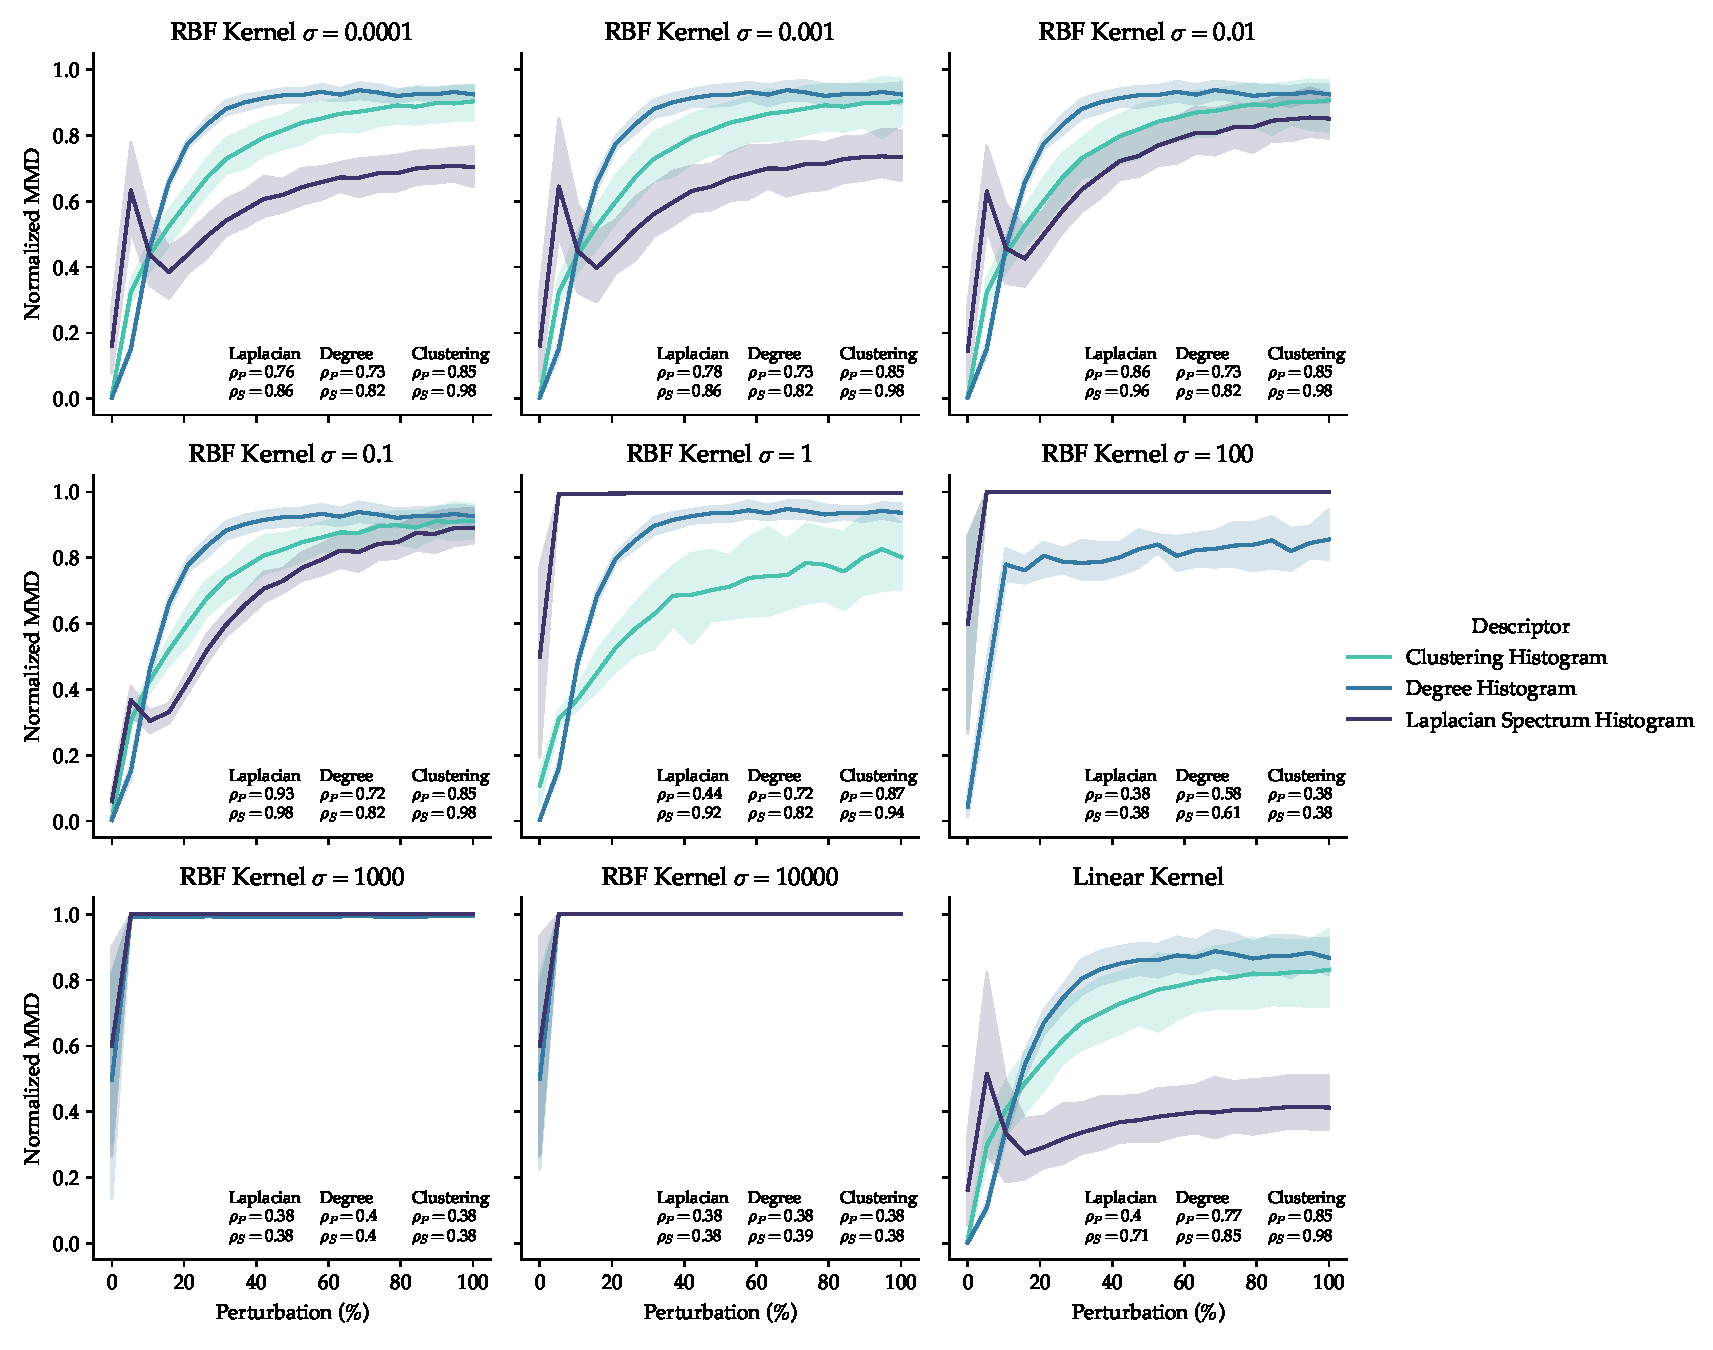
\includegraphics[width=\textwidth]{./figures/results/res_1_5.pdf}
  \caption[MMD vs. Gaussian Noise Perturbation (in \%) for various graph
descriptors of the 2-NN-graphs.]{MMD vs. Gaussian Noise Perturbation (in \%) for
various graph descriptors of the 2-NN-graphs. The kernel here is shown on top of
each subplots.}
  \label{fig:mmd_effect_kernel_knn}
\end{figure}


\section{Weisfeiler-Lehman Runtime Improvements for Sparse
  Graphs}\label{sec:sparse_wl}

In this thesis, we devised a three-pronged method to speed up the runtime of the
Weisfeiler-Lehman kernel by approximately 80\% by leveraging the sparsity of the
graphs used here. The three elements contributing to the speedup are the
following:

\begin{enumerate}
\item Our implementation parallelizes the execution of Weisfeiler-Lehman hash
computations since each graph's hash can be computed independently prior to
computing the kernel.
\item It also parallelizes the computation of similarity of graphs in RKHS by
computing batches of the inner products independently.
\item When comparing graphs, lots of CPU cycles are spent processing
positions/hashes that do not actually overlap between Weisfeiler-Lehman
histograms. As such, we manually loop over the overlapping keys, outperforming
numpy dot product-based implementations on collections of sparse graphs.
\end{enumerate}

We tested, covered, and open-sourced the implementation of this novel approach
on GitHub, and is available at the following URL: \url{https://github.com/pjhartout/fastwlk}.

\section{Distance Distribution of Descriptor Functions}
To explain why certain Gaussian configurations tend to work better than others,
it is useful to compute the pairwise distance of unperturbed proteins to get an
idea of how far away in e.g. Euclidean space, each embedding is from one
another.

\begin{figure}
  \centering
  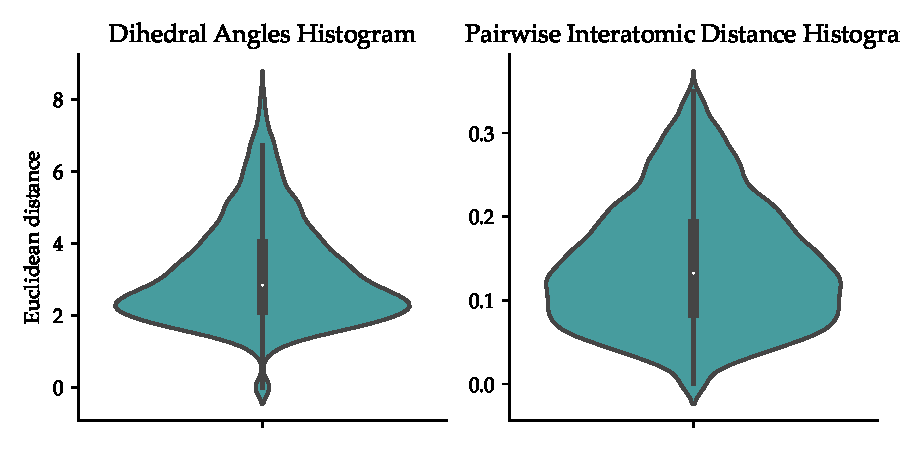
\includegraphics[width=0.6\textwidth]{./figures/results/violin_protein_descriptors.pdf}
  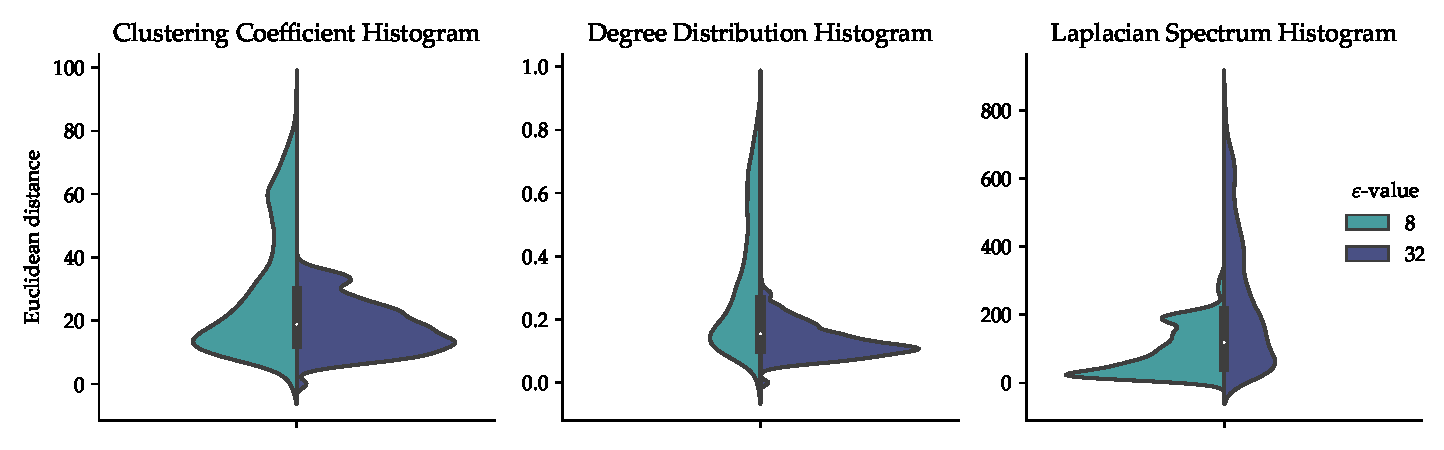
\includegraphics[width=\textwidth]{./figures/results/violin_graph_descriptors.pdf}
  \caption{Mean Euclidean distance between descriptor representations. The top
    row shows the mean distance between each of the protein descriptors
    introduced in this thesis while the bottom row shows the distance between
    each graph descriptor for two $\varepsilon$-graph extraction settings.}
\end{figure}


\backmatter

\bibliographystyle{plainnat}
\bibliography{refs}

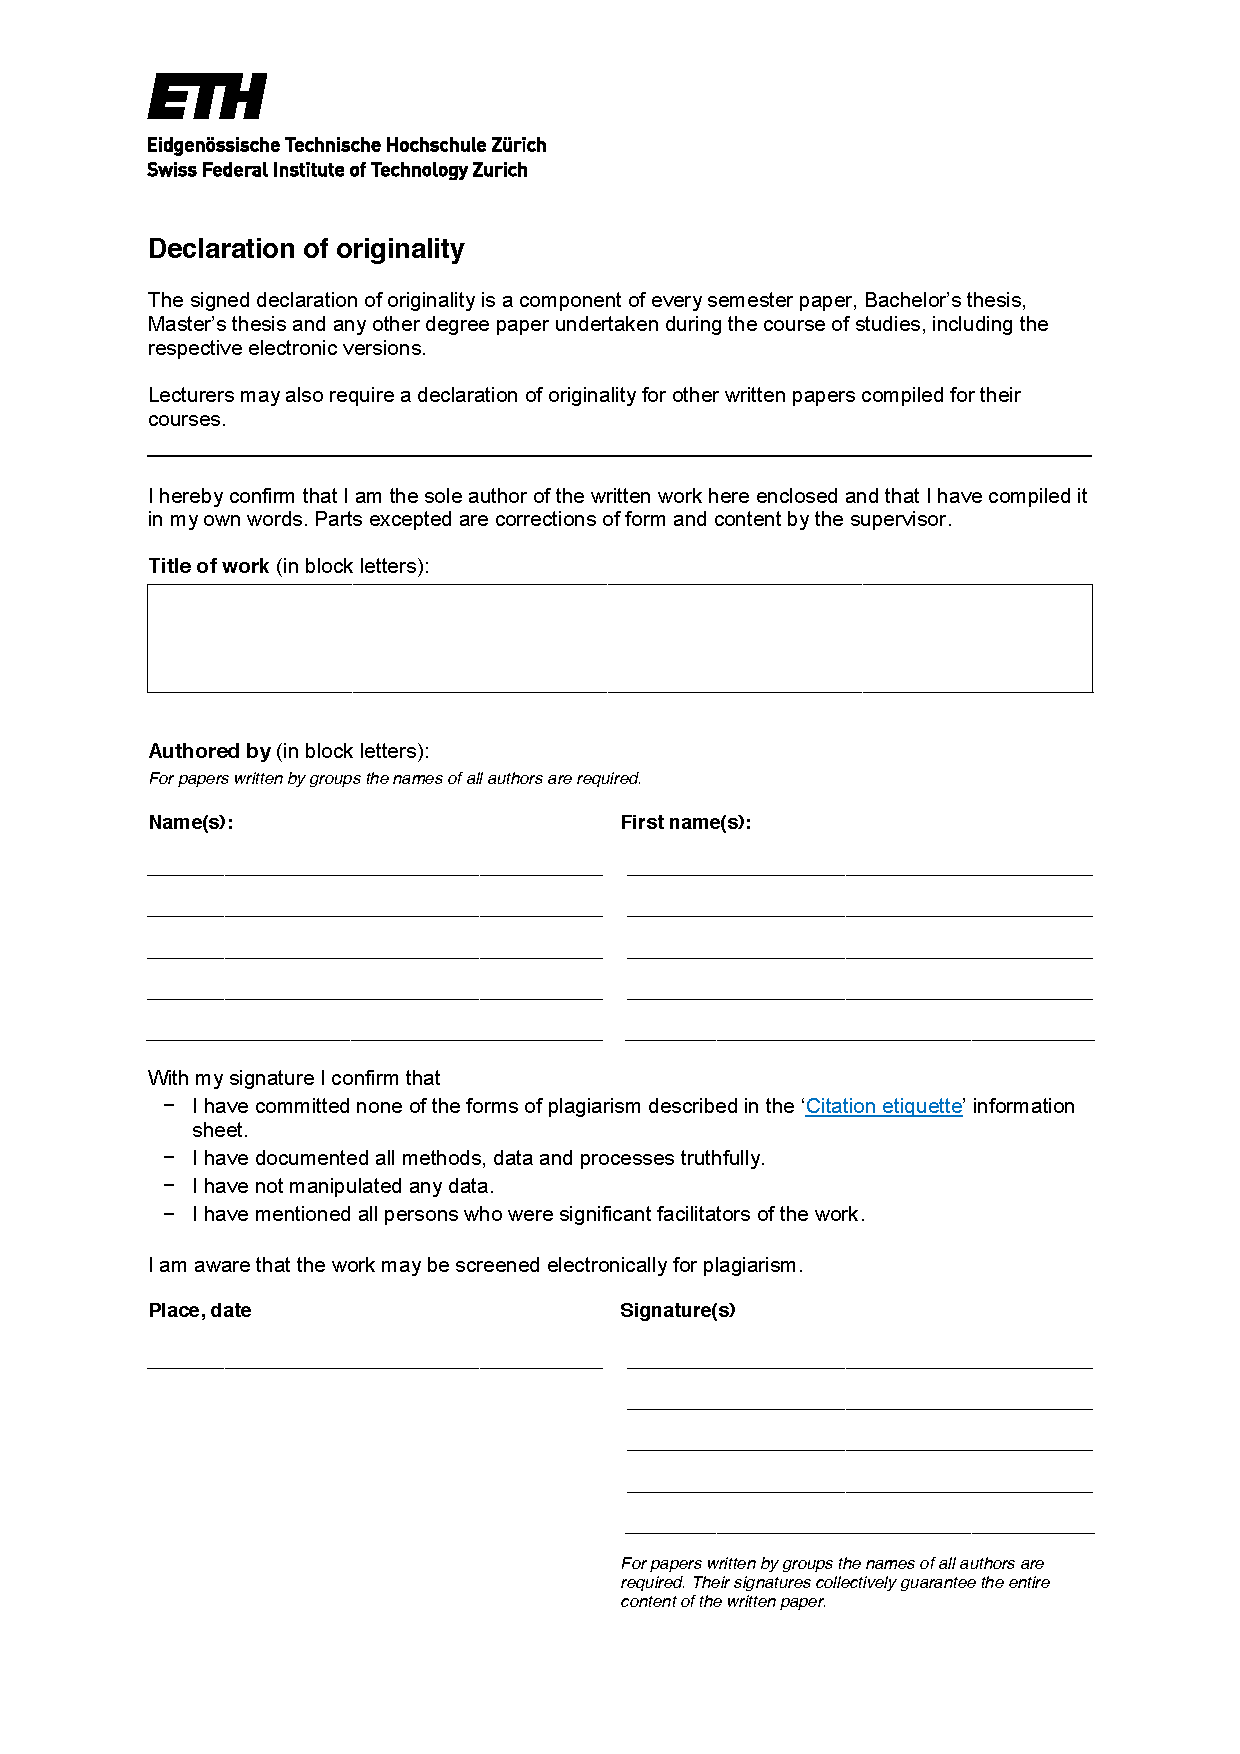
\includepdf[pages={-}]{declaration-originality.pdf}

\end{document}
